%%% CLASS SETTING %%%
\documentclass[letterpaper, 12pt]{article}
\usepackage{natbib}
\usepackage[margin=1in]{geometry} % sets page layout 
\bibpunct[, ]{(}{)}{,}{a}{}{,} % sets the punctuation of the bibliography entires.
\usepackage{authblk} 
\usepackage{url}

%%% Paper Information %%%
\title{When Strategic Uninformed Abstention Improves Democratic Accountability} 
\author{Gento Kato\thanks{Gento Kato is a Ph.D. Candidate, Department of Political Science, University of California, Davis, One Shields Avenue, Davis, CA 95616 USA (gkato@ucdavis.edu). The earlier version of this paper was presented at the 77th Annual Midwest Political Science Association Conference, Palmer House Hilton, Chicago, IL, April 5, 2019. The latest version of this paper is available from \texttt{https://github.com/gentok/UninformedModel}}}
\affil{University of California, Davis}
\date{Last Update: December 2, 2019}

% Other Packages/Settings
\usepackage{amsfonts, amsmath, amssymb, bm} %Math fonts and symbols
\usepackage[format=hang, justification=centering]{caption}
\usepackage{dcolumn, multirow} % decimal-aligned columns, multi-row cells
\usepackage{graphicx, subfigure, float} % graphics commands
\usepackage[colorlinks=true, citecolor=blue]{hyperref}
\usepackage{setspace}% allows toggling of double/single-spacing
\doublespace % set document spacing to double
%\usepackage{endnotes}
%\let\footnote=\endnote
% Draw figure
\usepackage{tikz}
\usetikzlibrary{calc}
% Add note to Figures
\newcommand{\floatnote}[1]{\vspace{\abovecaptionskip}\caption*{\textbf{Note:} #1}\vspace{-\abovecaptionskip}}
% Change section font
\usepackage{sectsty} 
\sectionfont{\fontsize{12}{12}\selectfont} 
\subsectionfont{\fontsize{12}{12}\selectfont} 
\subsubsectionfont{\fontsize{12}{12}\selectfont} 
% Move figures to the last
%\usepackage[figuresonly]{endfloat} %nomarkers, to avoid markers
\renewcommand{\listoffigures}{} % but suppress these lists

\begin{document}
    
    \begin{titlepage}
    
    \bibliographystyle{apsr}
    \maketitle
    \thispagestyle{empty}
    
    \clearpage
    \thispagestyle{empty}
    
    \begin{abstract}
        The recent development in formal studies of election makes two sets of findings that question the custom to treat voter information as a prerequisite for competent democratic decision-making. One argues that uninformed abstention is an effective strategy to approximate informed electoral outcome, and another suggests that uninformed voters may motivate strategic political elites to improve accountability. This article bridges and extends two findings by analyzing strategic incentives in the comprehensive voting model with abstention and its connection with electoral accountability. The proposed model offers a contextual explanation for two contrasting logic in uninformed abstention ---delegation and discouragement--- and shows that uninformed voting with abstention sometimes improves accountability. Furthermore, uninformed abstention is more effective in generating democratically preferred outcome under delegatory than discouraged context. The results make significant addition to the existing accountability literature by providing a more general mechanism by which less voter information improves policy outcomes.
    \end{abstract}
    \end{titlepage}
    
    \clearpage
    
    \par Empirical studies of voter competence often assume political information as the prerequisite for voters to make democratically competent decisions. As a result, many studies equate the evidence of ill-informed public with a dysfunctional democracy \citep{Converse1964thna, Dellicarpini1996wham, Bartels1996unvo, Somin1998voig, Achen2016defo}. Even in studies that do not consider information as the necessary condition for competent decisions, it is commonly assumed that acting \textit{as-if} informed is the end goal for uninformed voters to be democratically competent \citep{Lupia1994shve, Lupia2016unwh, Popkin1994thre, Boudreau2009clth}. However, the collection of findings from formal studies suggest that after incorporating strategic incentives in the election, \textit{uninformed voters} (who do not emulate informed decisions) \textit{do not necessarily hurt, and can even improve, the quality of democratic decision-making}. 

    \par Two major lines of formal argument challenge the assumption of incompetent uninformed voters. First, ideologically-neutral uninformed voters may abstain strategically to delegate the electoral outcome to the hands of ideologically-neutral informed voters \citep{Feddersen1996thsw,Feddersen1999abin}. Those studies show that ``informed'' electoral outcome does not need to be a product of fully-informed electorates. Second, low-information voting may induce the strategic reaction of political elites that benefit voters as a whole \citep{Ashworth2014isvo, Prato2016thvo}. Those studies suggest that uninformed voters have the potential to motivate elites and improve democratic accountability. Both arguments imply that it is misleading to equate information with vote competence, but under significantly different modeling approaches.
    
    \par This article thus aims to bridge previous formal findings on low-information voter competence by exploring strategic incentives in both uninformed abstention and elite accountability. At the baseline, I construct a simple model of referendum election with abstention. There are two representative groups of voters: informed and uninformed. One group of voters is randomly drawn by nature to be pivotal and determines the electoral outcome. In the election, voters first choose to participate or abstain. If participating, they can approve or reject the new policy proposal that replaces the status quo policy. The policy preference has two dimensions, the \textit{ideology} of voters and policy \textit{quality}. While each voter group has a prior ideology of liking or disliking the policy proposal, policy quality commonly benefits both voter groups. Informed and uninformed voters are different in their knowledge of policy quality. Informed voters know, while uninformed voters are uncertain, if the quality is high or low.
    
    \par While under a vastly simplified, less demanding setting, basic construct of the baseline model follows that of \cite{Feddersen1996thsw}. In the equilibrium election, highly ideological voters (denoted as \textit{ideologues} in the following) always participate, and vote based on ideology. Among non-ideologues, informed voters always participate, and vote based on policy quality. Non-ideologue uninformed voters are the only ones who may abstain from the election. Furthermore, to generalize the costless and instrumental voting model proposed in \cite{Feddersen1996thsw,Feddersen1999abin}, my model incorporates both the non-instrumental expressive benefit and minimal cost of voting. 

    \par The central results of the baseline model (Proposition 1) identify three mutually-exclusive contexts where the lack of information can lead to abstention: \textit{discouraged}, \textit{delegatory}, and mixed. Under discouraged abstention context, uninformed voters abstain when they fail to overcome the cost of voting due to a combination of uncertainty in policy quality and low pivotality. This abstention logic is consistent with the conventional decision-theoretic model of voting participation \citep{Downs1957anec, Riker1968thof, Matsusaka1995exvo}. Under delegatory abstention context, uninformed voters abstain when they benefit from informed voters monopolizing the electoral decision. When their pivotality in the election is high, independent of voting cost, uninformed voters are better off abstaining strategically to ensure that informed voters determine the electoral outcome than participating and making uncertain vote choices (Proposition 2). This abstention logic follows \cite{Feddersen1996thsw, Feddersen1999abin}. Both discouraged and delegatory abstention incentives are present under mixed abstention context. The results contribute to the literature by identifying contexts that differentiate the available logic of abstention.
    
    \par In the extended model, a third actor---the policymaker---endogenously proposes the policy to be voted in the election. In response to expected voter characteristics, he proposes either a high or low-quality policy. The similar model setting is used to assess electoral accountability \citep{Ashworth2014isvo, Prato2016thvo}.\footnote{The proposed model does not allow the policymaker to misrepresent himself in the election. Informed voters always learn the policy quality correctly, while uninformed voters never receive information regarding policy quality before they vote.} The policymaker varies in its capacity to formulate policy \citep{Gailmard2007slan, Huber2004buca}: the high-capacity type pays a lower cost to formulate a high-quality policy than the low-capacity type. 

    \par The central focus of the extended model is the decision of the policymaker. The low-capacity policymaker always prefers a low-quality policy, but the high-capacity policymaker may have an incentive to propose a high-quality policy with positive probability. The main results (Propositions 4 and 5) show the existence of a condition where the likelihood of a high-quality policy being proposed is increasing in the pivot probability of uninformed voters. This finding follows the suggestion in \cite{Ashworth2014isvo} that uninformed voters sometimes improve, rather than reduce, the accountability of the policymaker. 
    
    \par Further inquiry reveals the interesting consequences of the available logic of uninformed abstention. In the baseline voting model, allowing for uninformed abstention increase the likelihood of ``informed'' electoral outcome always under delegatory abstention context, but not always under discouraged or mixed abstention context (Proposition 3). Also, when uninformed voting improves policy accountability, the increase in the likelihood of a high-quality policy tends to be larger under the context of delegatory abstention than under that of discouraged abstention (Proposition 6 and 7). Both through approximating informed outcome and improving accountability, delegatory abstention, when available, tends to be more effective than discouraged abstention in increasing the policy welfare of non-ideologue uninformed voters.
    
    \par The final result (Proposition 8) shows that if uninformed voters can endogenously set the pivot probability, they often maximize the uninformed pivot probability to induce accountability improvement, if available. While it is rare, one condition in which this pattern breaks is when the non-instrumental expressive benefit is overly large. It implies that, under delegatory abstention context, where the non-instrumental expressive benefit is high, uninformed voters may have an incentive to avoid accountability improvement.  
    
    \par By exploring the connection between uninformed abstention and electoral accountability, this study makes a significant addition to the literature by providing a more general mechanism by which less voter information improves policy outcomes. When the representative voter is disaggregated into informed and uninformed groups, uninformed voters can sometimes use abstention as a strategic tool to delegate decision-making authority to informed voters. Less informed voter population improves accountability the most when the electoral context allows uninformed abstention to effectively manipulate the identity of the pivotal voter to be informed and ideologically-moderate. 
    %\par By exploring the connection between uninformed abstention and electoral accountability, this study makes a significant addition to the study of low-information voter competence. When the representative voter is disaggregated into informed and uninformed groups, the availability of different uninformed abstention logics explains how and when uninformed voters have the power to improve the accountability of political elites.
    
    \section*{Modeling Uninformed Abstention}
    
    \par Two types of formal models have been used to examine the role of information in voting with abstention. First, the models of costly and sincere voting \citep{Downs1957anec, Riker1968thof, Matsusaka1995exvo} suggest that the lack of information influences voting by uniformly reducing the expected benefit from participation. According to their logic, uninformed voters are discouraged from participation due to the combination of high uncertainty in preference and high voting cost. The models of costless and strategic voting \citep{Feddersen1996thsw, Feddersen1999abin} suggest very different logic of uninformed voting. Their equilibrium analysis reveals that uninformed voters have a strategic incentive to abstain, and delegate their votes to informed voters even without voting cost. If uninformed voters use the expected actions of other voters to guide their decisions under costless voting context, ``strategic voting and abstention'' of uninformed voters ``may lead to an informationally superior election outcome'' \citep[][418]{Feddersen1996thsw}.  
    
    \par The baseline model in this article simplifies and extends the previous models to get more intuitive and comprehensive picture of uninformed voting. To make the model simple, the proposed model treats voters as representative groups, not as individuals---informed and uninformed voter groups. The voters within each group share preferences and act uniformly as a group. Typically, the models that deal with the relationship between voters and political elites utilize a similar setting \citep[e.g.,][]{Little2015pran}. Also, the group-level utility function is frequently introduced in formal studies of electoral participation \citep{Morton1991grin, Schram1991whpe, Uhlaner1989ratu, Coate2004grru,Feddersen2006thof}. The group voting model reduces the number of actors compared to voting models with the collection of individual voters and simplifies the decision calculus. Voters are not expected to make complex calculations of their individual pivotality in the election. Instead, they are expected to make an intuitive conjecture of their group pivotality.
    
    \par Additionally, in the proposed model, voters are uncertain about the distribution of ideology and information in the society, details that are critical in determining the strategic incentives of uninformed voters. In \citeauthor{Feddersen1996thsw}'s model, all voters are assumed to know the exact proportions of ideological and informed voters. However, it is unrealistic to expect (especially for uninformed) voters to know such details about the society. Therefore, my model posits that voters know the distribution of information and ideology status only with a probability.
    
    \par To make the model comprehensive, as suggested by \cite{Downs1957anec} and \cite{Riker1968thof}, voting is modeled as costly. Also, participated voters receive some expressive benefit (i.e., the benefit of voting that is not instrumental to the election result) as a result of participation. Such variables are omitted in \cite{Feddersen1996thsw, Feddersen1999abin}. Then, as suggested by \cite{Feddersen1996thsw}, voting is modeled as strategic. Thus, voters make decisions based not only on their preferences but also on the expected decisions of other voters.
    
    \section*{Modeling Accountability}

    \par The extended model goes beyond the incentives of voters and analyzes the relationship between uninformed abstention and strategic incentives of political elites. Apart from voting, accountability is another major topic in the formal studies of domestic politics. Scholars have been examining bureaucratic and executive accountability to the legislative branch \citep[e.g.,][]{Gailmard2013lewh} and politicians' accountability to voters in elections \citep[e.g.,][]{Ashworth2012elac}. Those studies explore how institutional design and electoral context influence the strategic interaction between actors and consequently, the welfare of service recipients (i.e., legislative branch for bureaucratic accountability, voters for electoral accountability).
    
    \par Recent evidence in accountability studies suggests that voters who are fully informed about the actions of policymakers do not necessarily produce the best outcome \citep{Ashworth2014isvo, Prato2016thvo}. Similarly, non-transparent communication and seemingly irrational decision calculus can be effective in keeping accountability \citep{Patty2017expo,Gailmard2019prpr}. In particular, \cite{Ashworth2014isvo} argues that after considering the strategic incentive of reelection seeking incumbent politician, voters are sometimes better off being less informed. They model two candidates election with pre- and post-election periods. If voter is fully-informed, incumbent (if his preference different from voter) faces the choice between two extreme options: set voter preferred policy and sure to be reelected or set his preferred policy and sure to be voted out. For voter, the first option maximizes the pre-election payoff but minimizes the post-election payoff. The opposite pattern applies to the second option. Uninformed voter eases extremity in incumbent choices by introducing uncertainty in the electoral outcome. Under uninformed condition, in each of pre- and post-election, voter payoff is neither maximized nor minimized. In total, however, voter may obtain higher payoff under uninformed than informed condition.
        
    \par Electoral accountability models, including \cite{Ashworth2014isvo}, treat voter as one representative actor and thus cannot allow abstention in the election. Since uninformed abstention is a heavily discussed topic in formal models of election \citep{Matsusaka1995exvo, Feddersen1996thsw, Feddersen1999abin}, this is an important omission in existing accountability studies. By disaggregating voter and allowing for uninformed abstention, the electoral accountability model in this article adds significant insights to the connection between voter information and electoral accountability.\footnote{Some main implications (e.g., the policy quality improvement after less informed voters, the part of Proposition 5) still hold under the alternative setting that can be represented by one representative voter. On the other hand, the current model gives a more realistic and richer understanding of the connection between voter information and accountability. See Online Appendix C for more discussion of the alternative model.}
    
    \section*{The Voting Game}
    
    \par At the baseline, I analyze a referendum voting game, where voters directly vote to approve or reject a single policy proposal. After the election, the status quo policy will be replaced by the proposed policy only if the proposal wins the election. The quality of the proposed policy is chosen from $q \in \{-1, 1\}$ as follows. If $q=1$, the proposed policy is of high quality and, if $q=-1$, the policy is of low quality. The quality of the status quo policy is given as $0$. Therefore, voters gain utility by choosing a high-quality policy proposal ($q=1>0$) and lose utility from a low-quality policy proposal ($q=-1<0$).\footnote{The model can be equivalently defined with the status quo policy with quality chosen from $q \in \{-1, 1\}$ and new policy with expected quality $0$.}
    
    \par There are two groups of voters, $g \in \{I, U\}$, both act as unitary actors. $I$ are informed voters and $U$ are uninformed voters. $I$ know $q$ for sure, while $U$ only know the prior probability of a high-quality policy proposal, $\phi = Pr(q=1) \in [0, 1]$. Separate from information status, each group of voters holds ideology $\beta_g \in \mathbb{R}$, which influences their policy-specific preferences independent of policy quality. Regarding the relationship between information and ideology, informed voters are thought to have stronger and overarching ideologies than uninformed voters \citep{Converse1964thna, Achen2016defo} but recent empirical evidence suggests that, for a specific issue or policy field, uninformed voters can have an equally strong ideological preference as informed voters \citep{Goren2012onvo, Broockman2016apto}. Here, the election concerns one specific policy. Therefore, I follow the recent suggestions and model that the ideologies of informed and uninformed voters are independently drawn from the same continuous probability density function $f(\cdot)$.
    
    \par I denote the vote choice as $x_g \in \{0,1\}$ so that $x_g=1$ indicates the vote to accept the policy proposal and $x_g=0$ the vote to reject the policy proposal. The correct vote choice, $r_g$, is captured by the consistency between $x_g$ and voters' preferences. $r_g$ can be expressed as the function of policy quality $q$ and voters' policy-specific ideological preference $\beta_g$:
    \begin{align}
    r_g[q, \beta_g] &= \begin{cases}
    1 &\text{ if } q + \beta_g > 0 \\
    0 &\text{ if } q + \beta_g < 0  \\
    (q + 1)/2 &\text{ if } q + \beta_g = 0\\
    \end{cases}
    \end{align}
    \noindent The above function implies that, if the sum of proposed policy quality and ideology exceeds zero, approving the proposal is the correct choice. If the above sum is negative, rejection is the correct choice.\footnote{If the sum of the proposed quality and ideology is equal to zero, it is assumed that voters prefer to vote with the proposed quality (i.e., accept the policy if and only if the policy is of high-quality).}
    
    \par Additionally, the correct choice function suggests that, on some occasions, voter preferences are determined solely by the ideology. I call those voters \textit{ideologues}. If $\beta_g > 1$, then $r_g[q, \beta_g]$ is always $1$ regardless of $q$ (approval ideologues). Similarly, $\beta_g < -1$ then $r_g[q, \beta_g]$ is always $0$ (rejection ideologues). Remember that $\beta_g$ is randomly drawn from the continuous probability density function $f(\cdot)$. This distribution is common knowledge but the realized value of $\beta_g$ is private information. The probability of ideologues can be represented by the cumulative density function $F(\cdot)$ of $\beta$:
    \begin{align}
    \text{The probability of approval ideologues: } &\kappa_{a} = 1 - Pr(\beta \leq 1) = 1 - F(1)   \\
    \text{The probability of rejection ideologues: } &\kappa_{r} = Pr(\beta \leq -1) = F(-1)   
    \end{align}
    \noindent The remaining type of voters are the \textit{non-ideologues}. Non-ideologues may possess ideology, but ideology does not dominate their voting decisions, as they consider both policy quality and ideology to make their decisions. Assume that $1-\kappa_{a} - \kappa_{r} >0$. This condition implies that any voter group can be formed of non-ideologues with positive probability.
    
    \par In addition to the utilities from the electoral outcome, voters gain or lose utility from their actions in the election.  First, voters pay fixed cost $c \in \mathbb{R}^+$ to participate in the election.\footnote{Think of $c$ as the physical cost of voting, which is expected to be distributed independently from the information status. The main result holds when $c$ differs between voter groups.} Second, voters receive \textit{expressive benefit} $d > 0$ from participating in the election. Expressive benefit is weighted by how certain is the voted option matched with the correct preference (i.e., $Pr(x_g=r_g[q, \beta_g])$). 
    This conceptualization is similar to what is referred to as ``expressive utility'' or ``concern for policy'' in the formal literature \citep{Dewan2008thqu, Little2015pran}.\footnote{Certain expressive benefit can be given independently of the vote choice. In this game, this \textit{fixed} expressive benefit is incorporated in the cost term, $c$, because it reduces participation cost uniformly.} Additionally, assume $d \geq c$: this setting isolates the incentives for abstention under the minimal cost of voting in which ideologues and informed voters always vote (see Lemma 1 and 2).  
    %voting is costless for voters who are certain to make correct choice. This setting isolates the incentives for abstention under the minimal cost of voting.
    
    \par Now, I denote the voting participation action of each group of voters as $v_g \in \{0,1\}$ so that $v_g=1$ indicates participation and $v_g=0$ indicates abstention. Additionally, I define the electoral outcome of policy approval as $a=1$ and rejection as $a=0$. $\epsilon$ is a random noise in the new policy outcome with the expected value of 0. The utility functions of voters can be summarized as:
    \begin{align}
    u_g [a,q,\beta_g,d,c,v_g,x_g] &= a\{\beta_g + q + \epsilon\} + v_g \{d \times Pr(x_g=r_g[q, \beta_g]) - c \} \label{uf}
    \end{align}
    
    \par The sequence of the game is as follows. First, according to $\phi = Pr(q=1)$, the new policy is proposed with quality $q$. Second, both voter groups observe their ideology $\beta_g$, but only informed voters $I$ observe the proposed policy quality $q$. In the third step, $I$ and $U$ decide whether to vote for approval, for rejection, or abstain. At the end of the sequence, either $I$ or $U$ is exogenously selected as the pivotal group. $U$ is the pivotal group with probability $\pi \in [0, 1]$ and $I$ with probability $1-\pi$. $\pi$ is common knowledge to all voters. The vote cast by the pivotal group determines the electoral outcome. If the pivotal group abstains, the outcome is determined by the participating voter group. However, if both groups abstain, the policy stays at the status quo.\footnote{This election mechanism is similar to that of the random dictator game \citep{Morton2015whmo}.} In a real-world context, pivot probability $\pi$ is closely on correlation with the population of each voter group. Since the pivotal voter in plurality elections comes from the majority voter group, $\pi$ is equivalent to the likelihood of uninformed voters being the majority group in the society. Voters should also be able to recognize informed and uninformed voters in the society \citep{Huckfeldt2001thso}, but information regarding the exact population of informed and uninformed voters is rarely made available through public media channels (e.g., television, newspapers, radio); it is thus fair to expect that voters have a sense of, but are not certain about, the population of informed and uninformed voters. The pivot probability reflects the incomplete knowledge regarding the majority voter group in the society. Unless $\pi \in \{0, 1\}$, voters are unable to determine the pivot group with certainty.
    
    
    \par The decision-making in the voting game is one-shot and involves uncertainty. Therefore, the equilibrium of interest is a Bayesian Nash equilibrium. The equilibrium behavior of ideologues (i.e., $\beta_I < -1$ or $\beta_I > 1$) implies the following lemma:
    
    \noindent \textbf{Lemma 1}: \textit{The equilibrium strategy $\{x^*_g, v^*_g\}$ of ideologues is to participate in the election and vote in line with their ideology,\footnote{Assume that voters do not play a weakly dominated strategy (i.e., $x_g=1-(q+1)/2$ when $q = - \beta_g$.)}, or} 
    \begin{align}
    x^*_g &= \begin{cases}
    1 &\text{ if } \beta_g > 1 \text{ (approval ideologues)}\\
    0 &\text{ if } \beta_g < -1 \text{ (rejection ideologues)}
    \end{cases} \\
    v^*_g &= 1
    \end{align}
    
    \noindent Then, for non-ideologues (i.e., $\beta_g \in [-1, 1]$), the following result holds for those informed: 
    
    \noindent \textbf{Lemma 2}: \textit{The equilibrium strategy $\{x^*_I, v^*_I\}$ of non-ideologue informed voters (i.e., $\beta_I \in [-1, 1]$) is to participate in the election and vote in line with the policy quality, or} 
    \begin{align}
    x^*_I &= (1 + q)/2 \\ 
    v^*_I &= 1
    \end{align}
    
    \par Ideologues only need to know the ideology and non-ideologue informed voters only need to know the policy quality to determine their optimal actions. By contrast, non-ideologue uninformed voters face three uncertainties to determine their equilibrium strategy. The first is the uncertainty regarding the quality of the policy proposal ($\phi = Pr(q=1)$), the second is the uncertainty regarding the pivotal group that determines the electoral outcome ($\pi$), and the third is the uncertainty regarding the ideology of informed voters. Informed voters are approval ideologues with probability $\kappa_{a}$, rejection ideologues with probability $\kappa_{r}$, and non-ideologues with probability $1 - \kappa_{a} - \kappa_{r}$. Given the set of beliefs, $\phi$, $\pi$, $\kappa_{a}$, and $\kappa_{r}$, the equilibrium strategy of uninformed voters implies the following lemma:
    
    \noindent \textbf{Lemma 3}: \textit{In the voting game, the equilibrium strategy $\{v^*_U, x^*_U\}$ of non-ideologue uninformed voters (i.e., $\beta_U \in [-1, 1]$) can be represented by a threshold for the expected policy quality ($\phi$), or} 
    \begin{align}
    x^*_U &= 
    \begin{cases}
    1 & \text{if } \phi \geq \phi^*_x = \cfrac{1}{2} - \cfrac{\pi \beta_U}{2(\pi + d)}\\
    0 & \text{otherwise}
    \end{cases} \\
    v^*_U &= 
    \begin{cases}
    0 \text{ if } 
    &\phi \geq \phi^*_{v1x0} = min\left\{ \phi^*_x, \phi^*_{vr} = \cfrac{\pi \kappa_{a} (1-\beta_U) + d - c}{\pi (\kappa_{a} (1-\beta_U) + (1-\kappa_{r}) (1 + \beta_U))+ d} \right\} \\
    &\text{ and } \\ 
    &\phi < \phi^*_{v1x1} =max\left\{ \phi^*_x,  \phi^*_{va} = \cfrac{\pi (1 - \kappa_{a}) (1-\beta_U) + c}{\pi ((1-\kappa_{a}) (1-\beta_U) + \kappa_{r} (1 + \beta_U)) + d} \right\} \\
    1 &\text{otherwise}
    \end{cases} 
    \end{align}
    \noindent $\phi^*_x$ is the \textbf{approval threshold}. Non-ideologue uninformed voters prefer approval over rejection if and only if there exists the probability of a high-quality proposal reaching the approval threshold or higher values. The higher the $\phi^*_x$, the higher is the probability of a high-quality proposal $(\phi = Pr(q=1))$ required to make uninformed voters approve it. 
    %Two facts are evident from Lemma 3. First, $\phi^*_x$ is weakly decreasing in ideology $\beta_U$. The higher the ideology, the more attractive the new policy proposal becomes to uninformed voters. Second, the larger the value of expressive benefit $d$, the weaker the influence of $\beta_U$ on the approval threshold is (i.e., the threshold sticks to 0.5). However, a strong motivation to express the correct choice incentivizes uninformed voters to use the most conservative approval threshold, regardless of ideology, which is 0.5.
    
    \section*{The Logic of Uninformed Abstention}
    
    \par This section explores when and why uninformed voters have reason to abstain from the election. Lemmas 1 and 2 show that ideologue and non-ideologue informed voters have no reason to abstain; the only voters to abstain are non-ideologue uninformed voters. From Lemma 3, the interval between $\phi^*_{v1x0}$ and $\phi^*_{v1x1}$ is the \textbf{abstention interval} (i.e., $[\phi^*_{v1x0},  \phi^*_{v1x1})$). That is, non-ideologue uninformed voters have an incentive to abstain from the election when $\phi$ falls between $\phi^*_{v1x0}$ and $\phi^*_{v1x1}$. The wider this interval, the stronger the incentive for non-ideologue uninformed voters to abstain from the election.
    
    \begin{figure}[t!]
        \caption{Approval Threshold $\phi^*_x$ and Abstention Interval $[\phi^*_{v1x0},  \phi^*_{v1x1})$ Explain the Equilibrium Voting Behavior of Non-ideologue Uninformed Voters}
        \label{fig:abint}
        \begin{center}
            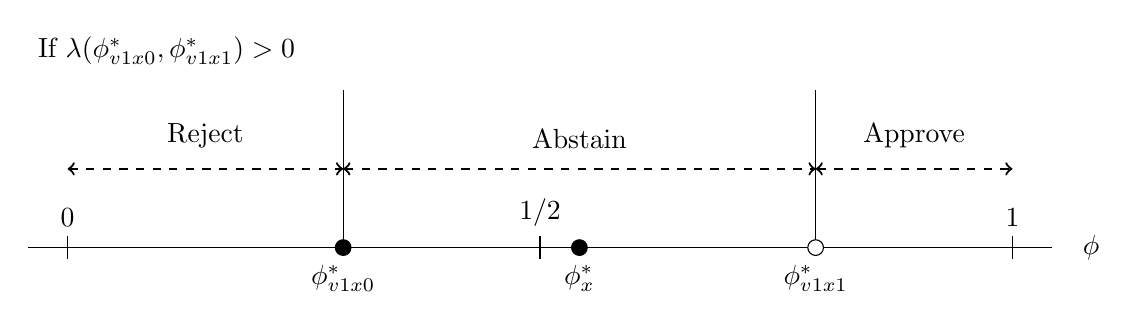
\begin{tikzpicture}
            \tikzstyle{solid node}=[circle,draw,inner sep=2,fill=black];
            \tikzstyle{hollow node}=[circle,draw,inner sep=2, fill=white];
            \draw (-6.5,0)--(6.5,0);
            \foreach \x in {-6,0,6} \draw (\x,0.15)--(\x,-0.15);
            \foreach \x in {-2.5,3.5} \draw (\x,0)--(\x,2);
            \node[above,yshift=4] at (-6,0) {$0$};
            \node[above,yshift=4] at (0,0) {$1/2$};
            \node[above,yshift=4] at (6,0) {$1$};
            \foreach \x in {-2.5,0.5} \node[solid node] at (\x,0) {};
            \foreach \x in {3.5} \node[hollow node] at (\x,0) {};
            \node at (7,0) {$\phi$};
            \node[below,yshift=-3] at (-2.5,0) {$\phi^*_{v1x0}$};
            \node[below,yshift=-3] at (0.5,0) {$\phi^*_{x}$};
            \node[below,yshift=-3] at (3.5,0) {$\phi^*_{v1x1}$};
            \draw[dashed, <->, thick] (-6,1)--(-2.5,1);
            \draw[dashed, <->, thick] (-2.5,1)--(3.5,1);
            \draw[dashed, <->, thick] (3.5,1)--(6,1);
            \node[above,yshift=4] at (-4.25,1) {Reject};
            \node[above,yshift=4] at (0.5,1) {Abstain};
            \node[above,yshift=4] at (4.75,1) {Approve};
            \node[right] at (-6.5,2.5) {If $\lambda(\phi^*_{v1x0},  \phi^*_{v1x1})>0$};            
            \end{tikzpicture}
        \end{center}
        \begin{center}
            \begin{tikzpicture}
            \tikzstyle{solid node}=[circle,draw,inner sep=2,fill=black];
            \tikzstyle{hollow node}=[circle,draw,inner sep=2, fill=white];
            \draw (-6.5,0)--(6.5,0);
            \foreach \x in {-6,0,6} \draw (\x,0.15)--(\x,-0.15);
            \foreach \x in {0.5} \draw (\x,0)--(\x,2);
            \node[above,yshift=4] at (-6,0) {$0$};
            \node[above,yshift=4] at (0,0) {$1/2$};
            \node[above,yshift=4] at (6,0) {$1$};
            \foreach \x in {0.5} \node[solid node] at (\x,0) {};
            \node at (7,0) {$\phi$};
            \node[below,yshift=-3] at (0.5,0) {$\phi^*_{v1x0}=\phi^*_{x}=\phi^*_{v1x1}$};
            \draw[dashed, <->, thick] (-6,1)--(0.5,1);
            \draw[dashed, <->, thick] (0.5,1)--(6,1);
            \node[above,yshift=4] at (-2.75,1) {Reject};
            \node[above,yshift=4] at (3.25,1) {Approve};
            \node[right] at (-6.5,2.5) {If $\lambda(\phi^*_{v1x0},  \phi^*_{v1x1})=0$};            
            \end{tikzpicture}
        \end{center}
        \floatnote{$\beta_U$ is assumed to be the negative value in this figure. $\beta_U=0$ implies that $\phi^*_x=1/2$ and $\beta_U>0$ that $\phi^*_x \leq 1/2$.}
    \end{figure}
    
    \par \autoref{fig:abint} visually illustrates the logic of uninformed abstention. The horizontal axis indicates the prior probability of a high-quality policy ($\phi$), and equilibrium behavior can be represented by the cut-points in $\phi$. I denote the width of the abstention interval as $\lambda(\phi^*_{v1x0},  \phi^*_{v1x1}) = \phi^*_{v1x1} - \phi^*_{v1x0}$. The top panel illustrates abstention behavior when $\lambda(\phi^*_{v1x0},  \phi^*_{v1x1}) > 0$. Under this condition, non-ideologues have an incentive to abstain from the election if $\phi$ falls between the lower bound ($\phi^*_{v1x0}$) and upper bound ($\phi^*_{v1x1}$ of the abstention interval. Given that $\phi^*_{v1x0} \leq  \phi^*_x \leq  \phi^*_{v1x1}$, the abstention interval always contains the approval threshold. If $\phi$ is lower than the lower bound (i.e., a low-quality policy is likely), non-ideologues participate and vote for rejection. However, if $\phi$ is higher than the upper bound (i.e., a high-quality policy is likely), non-ideologues participate and vote for approval. The bottom panel illustrates the voting logic when the width of the abstention interval is zero (i.e., $\lambda(\phi^*_{v1x0},  \phi^*_{v1x1}) =0$). Under this condition, non-ideologue uninformed voters always participate in the election and vote for approval or rejection, depending on the value of the approval threshold. 
    
    \par To understand the movement within the abstention interval, the following general result holds: 
    
    \noindent \textbf{Lemma 4}: \textit{The width of the abstention interval ($\lambda(\phi^*_{v1x0},  \phi^*_{v1x1})$) is weakly increasing in voting cost ($c$) and weakly decreasing in expressive benefit ($d$), probability of approval ideologues ($\kappa_a$), and probability of rejection ideologues ($\kappa_r$).}
    
    \noindent Lemma 4 shows behavioral patterns consistent with the previous studies on voting. Voting cost discourages participation, while expressive benefit encourages participation. Additionally, the motivation for participation is also increasing the likelihood of ideologues. Non-ideologue uninformed voters participate in the election when they believe informed voters are highly likely to be ideologues. This implication follows the argument in existing studies that voters with the minority preference tend to have a stronger motivation to participate in the election than those with majority preference \citep{Taylor2010puin, Cantoni2019pras}.
    
    \par In contrast to the above factors, the relationship between the pivot probability of uninformed voters and the abstention interval is conditional. The following proposition describes contexts that transform this relationship:
    
    \noindent \textbf{Proposition 1}: \textit{The lower bound of the abstention interval ($\phi^*_{v1x0}$) is weakly increasing in the uninformed pivot probability ($\pi$) if and only if the probability of ideologues is sufficiently high and the ratio of expressive benefit to voting cost ($d/c$) is sufficiently small, or}
    \begin{align}
    \frac{\kappa_{a} (1 - \beta_U)}{(1-\kappa_{r})(1+\beta_U)} > d/c - 1 \label{ecc1}
    \end{align}  
    \noindent \textit{Similarly, the upper bound of the abstention interval ($\phi^*_{v1x1}$) is weakly decreasing in the uninformed pivot probability ($\pi$) if and only if the probability of ideologues is sufficiently high and the ratio of expressive benefit to voting cost ($d/c$) is sufficiently small, or}
    \begin{align}
    \frac{\kappa_{r} (1 + \beta_U)}{(1-\kappa_{a})(1-\beta_U)} > d/c - 1 \label{ecc2}
    \end{align}
    
    \begin{figure}[t!]
        \caption{Visual Depiction of Discouraged and Delegatory Abstention Intervals}
        \label{fig:abgraph}
        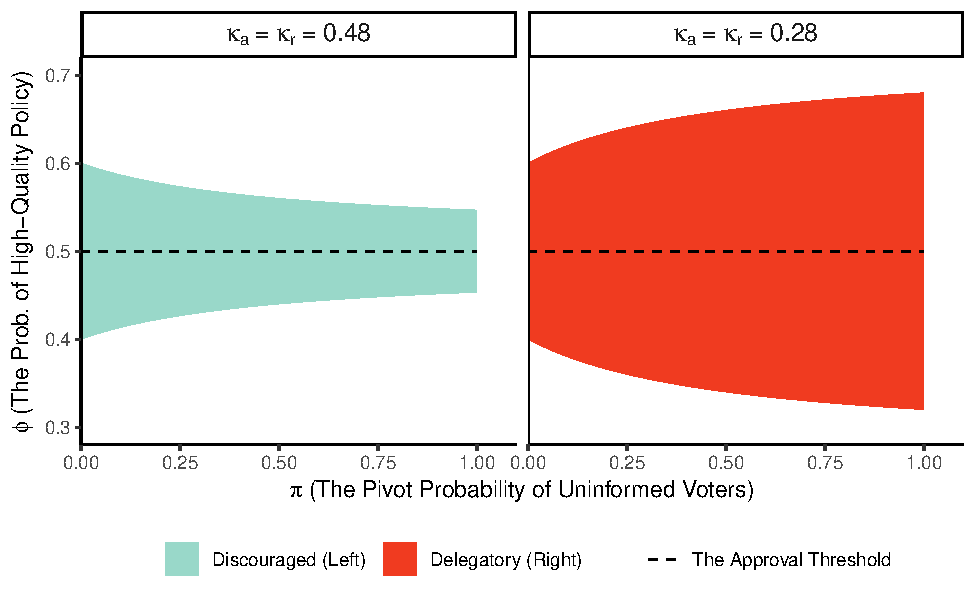
\includegraphics[width=\linewidth]{figure/abgraph-1}
        \floatnote{Other parameters are fixed at: $d=0.5$, $c=0.3$, and $\beta_U=0$.}
    \end{figure}
    
    \noindent Proposition 1 implies there are three possible relationships between the uninformed pivot probability and the abstention interval. \autoref{fig:abgraph} visually depicts the first two relationship forms. Here, the horizontal axis indicates the pivot probability of uninformed voters ($\pi$) and the vertical one the prior probability of a high-quality policy ($\phi$). Non-ideologue uninformed voters have an incentive to abstain from the election when $\phi$ falls within the shaded area. When both Inequalities \ref{ecc1} and \ref{ecc2} hold, the left-hand panel illustrates \textbf{discouraged abstention}: the abstention interval is narrowing in the uninformed pivot probability, both above and below the approval threshold. This form of abstention is called discouraged since the low probability of being pivotal in election dampens the motivation of non-ideologue uninformed voters to participate in the election. The logic resembles that of the traditional rational choice voting literature \citep{Downs1957anec, Riker1968thof, Matsusaka1995exvo}, in that the combination of low pivot probability, low expressive benefit, and high voting cost leads voters to abstain.
    
    \par When neither inequality \ref{ecc1} nor \ref{ecc2} holds, the right-hand panel illustrates \textbf{delegatory abstention}: the abstention interval is widening in the uninformed pivot probability, both above and below the approval threshold. This form of abstention is called delegatory because the logic is similar to that discussed in \cite{Feddersen1996thsw, Feddersen1999abin}. When the probability of being pivotal in the election is high, uninformed voters have the incentive to abstain strategically and \textit{delegate} the electoral outcome to informed voters. In other words, uninformed voters have an incentive to avoid making uncertain vote choices in the election and confuse the electoral outcome.
    
    \par The third type of abstention, \textbf{mixed abstention}, is a combination of the first two forms. When only inequality \ref{ecc1} holds, both the lower and upper bounds of the abstention interval are increasing in $\pi$. Similarly, if only inequality \ref{ecc2} holds, both the lower and upper bounds of the abstention interval are decreasing in $\pi$. Under mixed abstention condition, the abstention interval is narrowing in $\pi$ for one side of the approval threshold, but widening in $\pi$ for the other side of the threshold.  
        
    \begin{figure}[t!]
        \caption{$d:c$ Ratio and Probability of Ideologues $\kappa_a$, $\kappa_r$ Explain the Available Form of Abstention}
        \label{fig:abtype}
        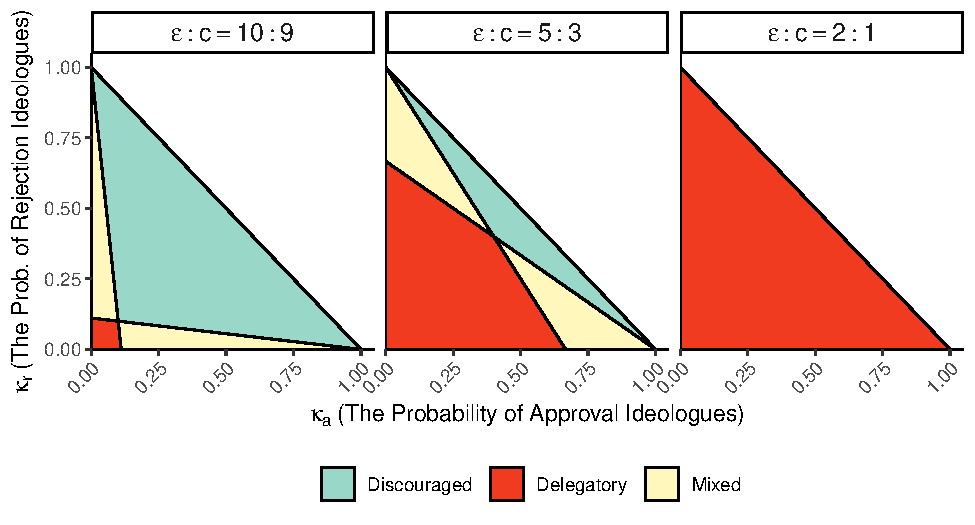
\includegraphics[width=\linewidth]{figure/abtype-1}
        \floatnote{$\beta_U$ is fixed at $0$. The absolute values of $d$ and $c$ can change, as long as the ratio holds. Additionally, since $\kappa_a + \kappa_r < 1$, the values of $\kappa_a$ and $\kappa_r$ falling within the upper right triangle of each panel do not exist.}
    \end{figure}
    
    \par The likelihood of ideologues ($\kappa_{a}$ and $\kappa_{r}$) and the ratio of expressive benefit to voting cost ($d/c$) play important roles in determining the form of the abstention for non-ideologue uninformed voters. \autoref{fig:abtype} summarizes these conditions. The shaded areas reflect the form of uninformed abstention possible under different values of $\kappa_a$ (horizontal axis), $\kappa_r$ (vertical axis). The dark (orange) shading indicates that abstention is delegatory, the brighter (green) shading indicates discouraged abstention, and the brightest (yellow) shading indicates mixed abstention. 
    
    \par Each panel of \autoref{fig:abtype} depicts the different ratios of $d$ to $c$. Across panels, the area of delegatory abstention is increasing, while the area of discouraged abstention is decreasing as ratio. Notice that when $c$ is sufficiently low relative to $d$, the only possible abstention type is delegatory (as shown in the rightmost panel). In fact, the following proposition holds for the existence of the abstention interval with a positive width (i.e., $\lambda(\phi^*_{v1x0},\phi^*_{v1x1})>0$):
    
    \noindent \textbf{Proposition 2}: \textit{When $c=0$, non-zero abstention interval (i.e., $\lambda(\phi^*_{v1x0},\phi^*_{v1x1})>0$) exists only under the context of delegatory abstention, for a sufficiently high $\pi$ and sufficiently low $\kappa_a$, $\kappa_r$, and $d$.}
    
    \noindent Proposition 2 follows the implications of \cite{Feddersen1996thsw}, who argue that delegatory abstention occurs independently of voting cost, while discouraged abstention is impossible under the no cost of voting. Note that the absolute value of $d$ must be sufficiently low to ensure the existence of a non-zero delegatory abstention interval. For delegatory abstention to occur, the expressive benefit to voting cost ratio (i.e., $d/c$) must be sufficiently high but the absolute difference between two parameters (i.e., $d-c$) must be sufficiently low. This pattern emerges because a high absolute non-instrumental utility reduces the relative importance of receiving instrumental utility from policy quality (which is fixed to $-1$ and $1$ in this game). If the absolute value of expressive benefit is too high, uninformed voters are better off voting than delegating even if the likelihood of the correct choice is low.
    
    \par In the left-hand and central panels of \autoref{fig:abtype} (i.e., voting cost is sufficiently high relative to expressive benefit), the prior probability of ideologues plays an important role in determining what form of abstention may occur. Inequalities \ref{ecc1} and \ref{ecc2} imply that, when voters are non-ideologues for sure (i.e., $\kappa_{a} = \kappa_{r} = 0$), only delegatory abstention is possible. Delegatory motivation leads to abstention when non-ideologue uninformed voters expect informed voters to share the same preference. An increase in the likelihood of ideologues makes discouraged abstention more likely than delegatory abstention. If informed voters are highly likely to be ideologues, non-ideologue uninformed voters lose the incentive to delegate votes. Under this condition, abstention occurs only due to discouragement from high voting cost. Mixed abstention tends to occur when the likelihoods of approval ideologues and of rejection ideologues differ significantly. If $\kappa_a$ is significantly higher than $\kappa_r$ (the bottom right corner of each panel), delegatory motivation drives abstention when non-ideologue uninformed voters relatively prefer the approval vote (i.e., $\phi \geq \phi^*_x$) and discouraged motivation drives abstention when non-ideologue uninformed voters relatively prefer the rejection vote (i.e., $\phi < \phi^*_x$). The opposite pattern occurs if $\kappa_r$ is significantly higher than $\kappa_a$ (the top left corner of each panel).
    
    \par The above uninformed voting logic unifies the two different explanations of uninformed abstention discussed in the literature. Discouraged abstention follows the classic logic of political participation \citep{Downs1957anec} to see abstention as the product of high voting cost and low electoral efficacy. Delegatory abstention supports the contrasting view suggested by \cite{Feddersen1996thsw} to understand uninformed abstention as the active delegation of the electoral decision to informed voters. Proposition 1 identifies electoral contexts that condition the occurrence of different abstention forms. When voting cost is sufficiently low and the likelihood of informed voters sharing the same preference as non-ideologue uninformed voters is sufficiently high, the abstention of non-ideologue uninformed voters occurs as a result of active delegation rather than discouraged inactivity.
    
    \par Lastly, consider if uninformed abstention helps to approximate the electoral outcome of fully-informed public. Define \text{informed outcome} as the hypothetical electoral outcome where both $I$ and $U$ are informed. The following proposition holds for the likelihood of informed outcome.   
    
    \noindent \textbf{Proposition 3}: \textit{Under the context of delegatory abstention, allowing for uninformed abstention always weakly increases the likelihood of informed outcome. However, under contexts of discouraged and mixed abstention, there exists a condition where allowing for uninformed abstention decreases the likelihood of informed outcome.}
    
    \noindent Proposition 3 shows that uninformed abstention is not always helpful in approximating the informed electoral outcome. Following \cite{Feddersen1996thsw}, delegatory abstention always improves the likelihood of a high-quality policy being approved and a low-quality policy being rejected. On the other hand, if the available form of abstention is either discouraged or mixed, uninformed abstention may not be helpful in approximating the informed electoral outcome. Rather, uninformed voters abstain for the sake of non-instrumental gain from not paying voting cost.
    
    \section*{The Accountability Game}
    
    \par Here, I extend the voting game to consider the situation where the proposed policy quality is endogenously determined by a third actor. I call this new game the accountability game. For simplicity, assume that the ideology is chosen from three discrete categories ($\beta_g \in \{R, 0, A\}$ where $R<-1$ and $A>1$).\footnote{This is a special case of the ideology distribution $f(\cdot)$. The central implications hold with a more general $f(\cdot)$.} This game inherits almost all settings of the voting game but has an additional stage at the beginning: the $P$ proposes policy proposal $q$.
    
    \par Formal studies on policymaking suggest that a policymaker may have a differential capacity to formulate a high-quality policy \cite[e.g.,][]{Gailmard2007slan, Huber2004buca}. As such, in the accountability game, there are two types of policymakers $T \in \{H, L\}$: the high-capacity $P_H$ and low-capacity $P_L$. The two types differ in the level of effort required to formulate the policy. The high-capacity policymaker puts relatively low effort $\eta_H = 1$ to achieve the high quality compared to the low-capacity policymaker (who needs $\eta_L = 2$ to achieve a high-quality policy). Further, the policymaker gains a fixed positive benefit ($B=2$) from the new policy being approved in the election.\footnote{The default values normalize the cost of policymaking. The central implications hold as long as $\eta_H < B \leq \eta_L$.} One can understand $B$ as the motivation for policymakers to appear effective in creating the policy. Consequently, the utility function of $P$ is defined as:
    \begin{align}
    u_P = \begin{cases}
    2 - \eta_T \cdot (1+q)/2 &\text{ if the policy is approved} \\
    - \eta_T \cdot (1+q)/2 &\text{ if the policy is rejected} \\
    \end{cases} \label{acuf}
    \end{align}
    \noindent Regardless of the electoral outcome, the policymaker has to put effort $\eta_T$ into formulating a high-quality policy ($q=1$). On the other hand, a low-quality policy can be formulated without this effort. Then, if the policy is approved, the policymaker receives approval benefit $B=2$. 
    
    \par The utility function represented in \autoref{acuf} implies the following lemma regarding the equilibrium decision of the low-capacity policymaker:
    
    \noindent \textbf{Lemma 5}: \textit{The equilibrium strategy of the low-capacity policymaker $P_L$ is to always propose a low-quality policy ($q=-1$).}
    
    \noindent Lemma 5 shows that the low-capacity policymaker always proposes a low-quality policy ($q=-1$) at equilibrium. The approval benefit ($B=2$) fails to make up for the effort level required for a high-quality policy ($\eta_L=2$). This assumption implies that $p$ represents voters' uncertainty regarding whether the policymaker is responsive in the election: Only the high-capacity policymaker is potentially responsive to their voting strategies. 
    
    \par The type of the policymaker is not common knowledge, and all voters form belief $p \in [0, 1]$, which indicates the probability of the high-capacity policymaker. Since the low-capacity policymaker always proposes a low-quality policy (Lemma 5), voters are only uncertain about the decisions of the high-capacity policymaker. I denote $\phi_H \in [0,1]$ as the probability that the high-capacity policymaker formulates a high-quality policy. Given that only the high-capacity policymaker can potentially formulate a high-quality policy, voters' prior belief regarding the probability of high-policy quality is represented by $\phi = p \cdot \phi_H$. 
    
    \par The sequence of the accountability game is as follows. First, nature selects the high-capacity policymaker with probability $p$ and the low-capacity policymaker with $1-p$. $p$ is common knowledge. Then, the selected policymaker ($P_T$) decides whether to propose a high- or low-quality policy by $\phi_T = Pr(q=1) \in [0, 1]$. Only informed voters observe the quality of the policy. If $\phi_T = 0$, the policymaker of type $T$ proposes a low-quality policy for sure; if $\phi_T = 1$, the policymaker of type $T$ proposes a high-quality policy for sure. The election in the accountability game is identical to the voting game. 
    
    \par Since the accountability game involves the dynamic process of decision-making, the appropriate equilibrium of interest is a perfect Bayesian equilibrium. The analytical result of the voting game (Lemmas 1--3) still explains the equilibrium behavioral rule of voters because two games share the same voting process. The focus of this section is describing the behavior of the policymaker. To establish the baseline behavior, suppose that informed voters are always pivotal in determining the electoral outcome ($\pi=0$). The following proposition reflects the equilibrium behavior of the high-capacity policymaker:
    
    \noindent \textbf{Proposition 4}: \textit{Suppose that $\pi=0$. $P_H$ proposes a high-quality policy for sure if the probability of ideologues is sufficiently low and a low-quality policy for sure otherwise, or}
    \begin{align}
    \phi^*_H[\pi=0] &=
    \begin{cases}
    0 &\text{ if }  \kappa_{a} + \kappa_{r} \geq 0.5 \\
    1 &\text{ if }  \kappa_{a} + \kappa_{r} < 0.5
    \end{cases}
    \end{align}
    
    \noindent Proposition 4 provides the starting point of the analysis when informed voters determine the electoral outcome for certain. This condition is equivalent to a fully-informed public because all voters who are potentially pivotal in the election are informed. Then, the likelihood of ideologues fully determines the quality decision of the high-capacity policymaker. If the combined likelihood of voters being ideologues (i.e., both approval and rejection ideologues) is below $0.5$, $P_H$ proposes a high-quality policy for certain ($\phi^*_H[\pi=0]=1$) thus fully-informed public maximizes the accountability. On the other hand, if the likelihood of ideologues is $0.5$ or above, $P_H$ proposes a low-quality policy for certain ($\phi^*_H[\pi=0]=0$). The high likelihood of ideologues dampens the motivation for a high-quality proposal because the decision calculus of ideologues cannot be influenced by the policy quality (Lemma 1). 
        
    \par The presence of potentially pivotal uninformed voters ($\pi>0$) changes the strategic motivation of the high-capacity policymaker. When $\phi^*_H[\pi=0]=1$, it is obvious that this change can only lead to a decline in accountability. Consistent with the existing arguments that information (or informed decision) is crucial for voters to become competent, for some positive $\pi$, $\phi^*_H$ moves down from $1$ (see Online Appendix B for the example).

    \par However, when $\phi^*_H[\pi=0]=0$, the following proposition holds for the decision of the high-capacity policymaker.
    
    \noindent \textbf{Proposition 5}: \textit{Suppose that $\phi^*_H[\pi=0]=0$ holds (i.e., $\kappa_{a}+\kappa_{r} \geq 0.5$). If $\pi>0$ (i.e., uninformed voters are potentially pivotal), $\phi^*_H$ deviates to $\phi^*_{v1x0}/p$ or $\phi^*_{v1x1}/p$ for a:
    \begin{itemize}
        \item sufficiently high $\pi$ with
        \item sufficiently high $p$ and 
        \item sufficiently low  $\kappa_{a}+\kappa_{r}$
    \end{itemize}
    }    
    
    \noindent In the above, the deviation from $\phi^*_H=0$ occurs because the increase in $\phi^*_H$ can increase the policy approval likelihood. By setting $\phi^*_H=\phi^*_{v1x0}/p$, the policymaker can ensure that the non-ideologue uninformed voters abstain from the election (instead of voting for rejection) and by setting $\phi^*_H=\phi^*_{v1x1}/p$ the policymaker can gain the approval vote of non-ideologue uninformed voters.
    
    \par Proposition 5 implies that the presence of potentially pivotal uninformed voters can increase the likelihood of high-quality policymaking, the finding consistent with \cite{Ashworth2014isvo}. When voters are fully-informed, the high-capacity policymaker facing a likely-to-be ideological population loses motivation to formulate a high-quality policy. However, under the equally ideological population with potentially pivotal uninformed voters, the high-capacity policymaker may have an incentive to set a high-quality policy with positive probability so that he can prevent the rejection vote of non-ideologue uninformed voters.
    
    \par Accountability improvement occurs under three conditions. First, the uninformed pivot probability ($\pi$) must be sufficiently high so that the prevention of their rejection votes is effective in increasing the policy approval likelihood. Second, the prior probability of the high-capacity policymaker ($p$) must be sufficiently high. When $p$ is too low, no possible value of $\phi_H$ can stop rejection votes of non-ideologue uninformed voters. Third, the likelihood of ideologues ($\kappa_{a}+\kappa_{r}$) must be sufficiently low. It must be $\kappa_{a}+\kappa_{r} \geq 0.5$ for accountability improvement to occur, but if it is too high, the expected decision of non-ideologue voters is not important in determining the electoral outcome.
    
    \par Moreover, consider the role of abstention logic in accountability improvement. When $P_H$ has an incentive to deviate from a low-quality policy ($\phi^*_H=0$), the following proposition holds for the equilibrium choice of the probability of high-quality policymaking:
    
    \noindent \textbf{Proposition 6}: \textit{Suppose that $\kappa_{a}+\kappa_{r} \geq 0.5$ and $P_H$ deviates from $\phi^*_H=0$ under $\pi>0$. Holding other factors constant, the choice of $\phi^*_{v1x0}/p$ tends to occur under discouraged abstention context (i.e., low $d:c$ ratio) and the choice of $\phi^*_{v1x1}/p$ under delegatory abstention context (i.e., high $d:c$ ratio).}
    
    \noindent Proposition 6 implies that the improvement in accountability induced by uninformed voting tends to be larger under delegatory than discouraged abstention context. Under delegatory abstention context, $P_H$ tends to propose a high-quality policy with a high probability to obtain the approval vote of non-ideologue uninformed voters. However, under discouraged abstention context, $P_H$ tends to propose a high-quality policy with low probability because he is better off suppressing than encouraging the participation of non-ideologue uninformed voters.
    
    \begin{figure}[t!]
        \caption{How The Presence of Uninformed Voters Improves Accountability}
        \label{fig:eupgraph}
        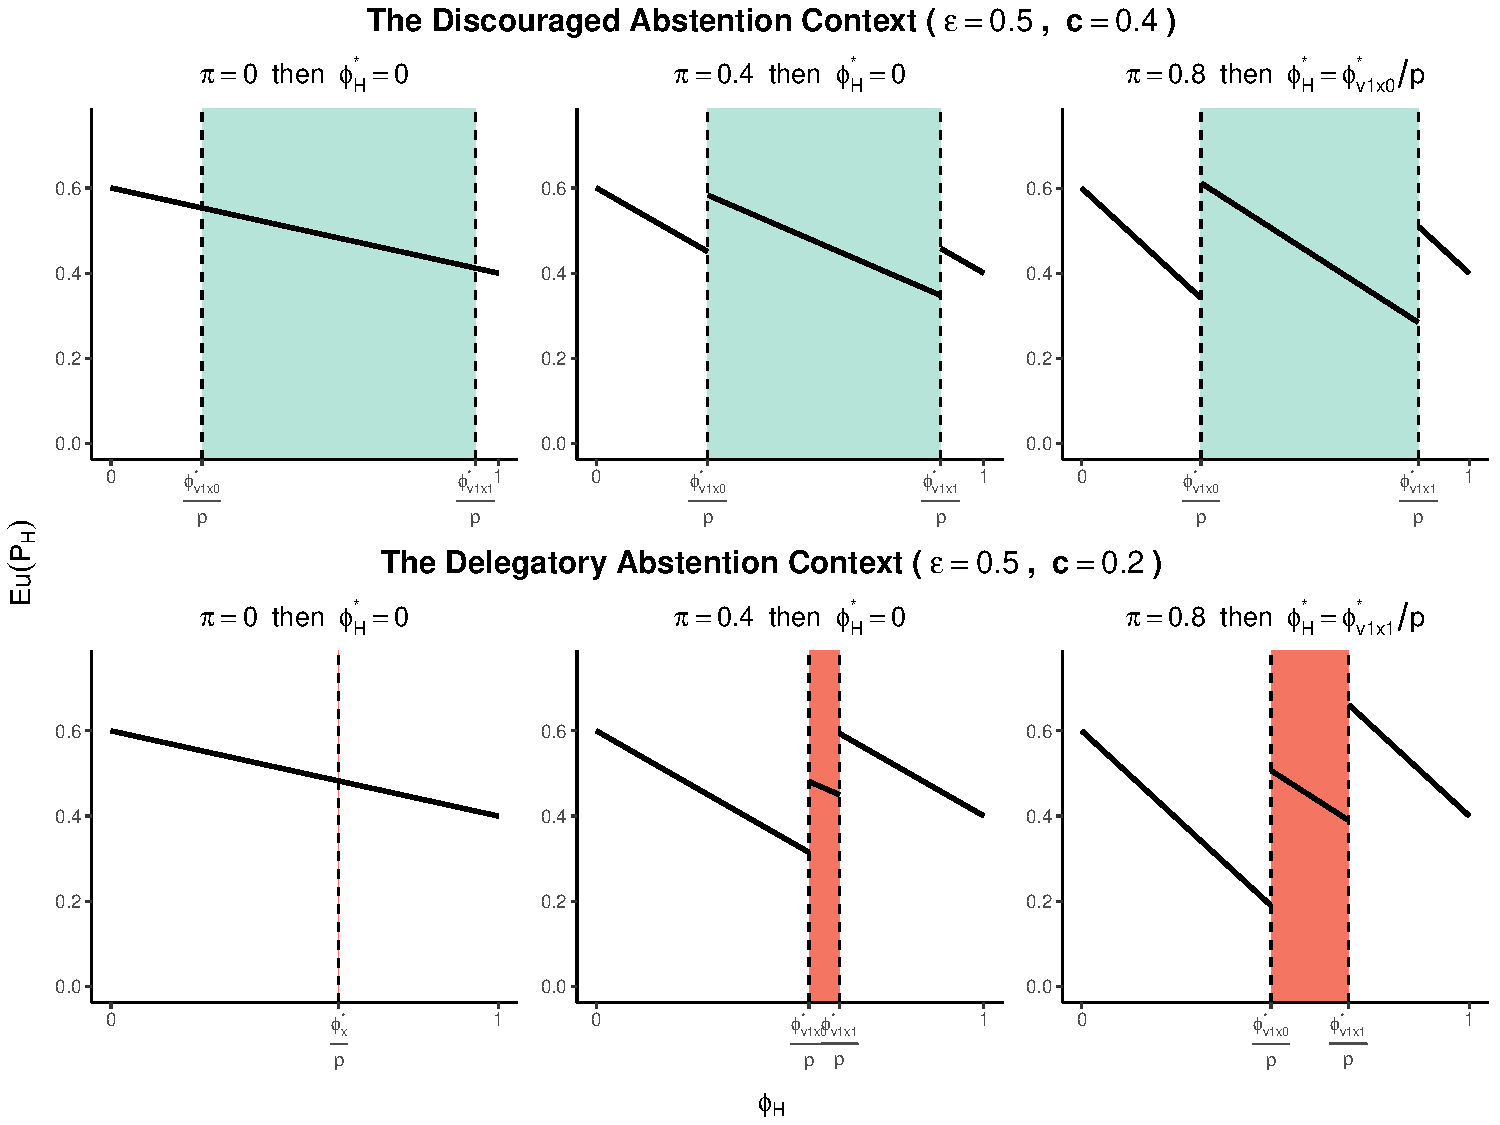
\includegraphics[width=\linewidth]{figure/eupgraph-1}
        \floatnote{Relevant parameters are fixed to: $\kappa_a = \kappa_r = 0.3$ and $p=0.85$. If $\phi_H$ falls within the shaded interval, non-ideologue uninformed voters abstain from the election.}
    \end{figure}
    
    \par \autoref{fig:eupgraph} illustrates the relationship between the decision calculus of $P_H$ and the presence of potentially pivotal uninformed voters when $\kappa_{r}+\kappa_{a}\geq 0.5$. %In each panel, the horizontal axis shows the policy quality decisions of the high-capacity policymaker ($\phi_H \in [0,1]$) and the vertical axis the corresponding expected utilities ($Eu(P_H)$). The equilibrium quality decision ($\phi^*_H$) is determined by the value of $\phi_H$ that maximizes expected utility. The figure focuses on the role of $\pi$ and the form of abstention in changing the equilibrium decision (other parameters are fixed at $\kappa_{r}=\kappa_{a}=0.3$ and $p=0.85$). The shaded area represents the values of $\phi_H$ that motivate non-ideologue uninformed voters to abstain from the election (i.e., corresponds to the interval illustrated in \autoref{fig:abint}). They cast a rejection vote for $\phi_H$ at the left-hand side of the interval and approval vote for $\phi_H$ at the right-hand side of the interval. %\par 
    In each row, the left panel shows $Eu(P_H)$ is strictly decreasing in the probability of a high-quality policy proposal ($\phi_H$). Facing the fully-informed pivotal voter ($\pi=0$), $P_H$ has no incentive to deviate from a low-quality policy. The central panel indicates that, if uninformed voters are potentially pivotal ($\pi>0$), $Eu(P_H)$ is increasing in $\phi_H$ at the cut-points that correspond to the change in uninformed voting behavior. If $\pi$ is sufficiently high (the right-hand panel), expected utility of $P_H$ is maximized at $\phi^*_H>0$.
    
    \par The top row of the figure illustrates the decision calculus when the available form of abstention is discouraged (i.e., high $d:c$ ratio, $d=0.5$ and $c=0.4$). In this case, the reduction in the abstention interval causes a more substantial increase in the $Eu(P_H)$ at the cut-point corresponding to the lower bound of the abstention interval (i.e., $\phi^*_{v1x0}$) than at the cut-point corresponding to the upper bound. The bottom row shows the opposite case. Under the electoral context with the delegatory abstention (i.e., high $d:c$ ratio, $d=0.8$, and $c=0.4$), the expansion of the abstention interval causes a more significant increase in $Eu(P_H)$ at the upper bound of the interval than at the lower bound. Consequently, for a sufficiently high $\pi$, $P_H$ proposes a high-quality policy with the higher probability under delegatory than discouraged abstention context.
    %\par Note that the prior probability of the high-capacity policymaker ($p$) plays a role in the decision calculus of $P_H$. The increase from $\phi^*_H=0$ occurs only when $p$ is sufficiently high. The logic behind this fact is as follows. First, the high-capacity policymaker proposes a high-quality policy with a positive probability only when this action can prevent uninformed voters from voting for rejection. Second, uninformed voters stop voting for rejection only when the prior belief of a high-quality policy proposal (i.e., $\phi = p \cdot \phi_H$) is sufficiently high. Since the low-capacity policymaker never proposes a high-quality policy, a low $p$ dampens the probability of a high-quality policy in general. When $p$ is low (i.e., $p < \phi^*_{v1x0}$), no possible value of $\phi_H$ can convince non-ideologue uninformed voters to stop voting for rejection; thus, $P_H$ sticks to a low-quality policy.
    
    \begin{figure}[t!]
        \caption{The Prevalence of Accountability Improvement in Response to Uninformed Voting}
        \label{fig:rangegraph}
        \includegraphics[width=\linewidth]{figure/rangegraph-1}
        % \floatnote{$c = 0.4$ and $\kappa_a=\kappa_r$ by assumption.}
    \end{figure}

    \par To illustrate the prevalence of accountability improvement, \autoref{fig:rangegraph} shows the pattens of $P_H$'s equilibrium policy decision ($\phi^*_H$) for realistic values of $\pi$, $p$, $d$, and $\kappa_a + \kappa_r$ under $\kappa_a + \kappa_r\geq0.5$.\footnote{$c$ is fixed to 0.4 and $\kappa_a=\kappa_r$ by assumption. See Online Appendix D for the illustration of accountability improvement availabilities over different values of those parameters.} In each panel, the horizontal axis indicates the size of expressive benefit ($d$. $c$ is fixed to $0.4$), which ranges from $0.45$ (only slightly higher than $c$) to $0.95$ (almost as large as the policy quality benefit/loss $|q|=1$), and the vertical axis indicates the uninformed pivot probability $\pi$. The dark (orange) shaded area indicates accountability improvement to $\phi_{v1x1}/p$, the light (green) shaded area indicates accountability improvement to $\phi_{v1x0}/p$, and remaining white area indicates no accountability improvement ($\phi^*_{H}=0$) in the equilibrium. As discussed in Proposition 5 and 6, accountability improvement may at higher values of $\pi$, $\phi^*_H=\phi_{v1x1}/p$ tends to occur under delegatory context (high $d:c$ ratio) and $\phi^*_H=\phi_{v1x0}/p$ tends to occur under discouraged context (low $d:c$ ratio).

    \par Comparing across panels in \autoref{fig:rangegraph}, the probability of the high-capacity policymaker ($p$, columns) and the likelihood of ideological voting ($\kappa_a+\kappa_r$, rows) play key roles in explaining the prevalence of accountability improvement. First, under high $p$ ($p=0.95$) and low $\kappa_a + \kappa_r \geq 0.5$ ($\kappa_a=\kappa_r=0.26$), accountability improvement occurs for the wide range of $\pi$ and $d$. Under this condition, accountability improvement is not rare: the minimal value of $\pi$ can induce $P_H$ to deviate from $\phi^*_H=0$. Then,as $p$ decreases and $\kappa_a + \kappa_r$ increases, the higher value of $\pi$ is required to induced accountability improvement, especially under contexts with intermediate $d$. For $p$ as low as $0.75$ or $\kappa_a+\kappa_r$ as high as $0.75$ (i.e., $\kappa_a=\kappa_r=0.35$), the presence of uninformed voters rarely induces accountability improvement.\footnote{$p=0.75$ may seem too high to be the lower bound of $p$. However, considering that the low capacity policy maker never responds to voters (Lemma 5), the high likelihood of $p$ is not unrealistic.}

    \par Lastly, the following proposition holds for the equilibrium decision of the high-capacity policymaker if uninformed abstention is not allowed. 
    
    \noindent \textbf{Proposition 7}: \textit{Suppose that $\kappa_a+\kappa_r \geq 0.5$ and uninformed abstention is not allowed. If $P_H$ deviates from $\phi^*_H=0$ under $\pi>0$, he chooses $\phi^*_x/p=1/2p$.}  

    \noindent The combination of Proposition 6 and 7 implies that if uninformed voting induces accountability improvement, allowing for abstention may increase or decrease the size of improvement. Since $\phi^*_{v1x0} \leq \phi^*_x \leq  \phi^*_{v1x1}$, allowing for abstention further improves accountability if $\phi^*_H=\phi^*_{v1x1}/p$ (tends to occur under delegatory abstention context) but reduces accountability if $\phi^*_H=\phi^*_{v1x0}/p$ (tends to occur under discouraged abstention context). Again, it is shown that uninformed voting contributes to the improvement in democratic decision-making especially under the context of delegatory abstention.
    %\par The analysis in this section shows that uninformed voting has the potential to improve policy accountability. The improvement occurs when the policymaker expects voters to be sufficiently ideological (i.e., $\kappa_{r}+\kappa_{a}\geq0.5$), he proposes a low-quality policy at no cost if all pivotal voters are fully-informed; however, he may pay the cost to formulate a high-quality policy if uninformed voters are potentially pivotal. Furthermore, if the policymaker proposes a high-quality policy with positive probability, this probability tends to be higher in electoral contexts where the available form of uninformed abstention is delegatory rather than discouraged.
    
    \section*{The Endogenous Selection of the Uninformed Pivot Probability}

    \par In the accountability game, the pivotal probability of uninformed voters ($\pi$) is set exogenously. However, in reality, uninformed voters may have tools to influence $\pi$ on their own prior to the occurrence of any specific elections (e.g., voter registration). To consider the implication of the endogenous $\pi$ selection, this section discusses the alternative formulation of the extended game in which $U$ has an opportunity to endogenously determine $\pi$ prior to the election (i.e., before anyone observing $\phi^*$ or $\beta_g$). Under this revised setting, the following proposition holds for the equilibrium selection of $\pi=\pi^*$. 
    
    \noindent \textbf{Proposition 8}: \textit{In the revised game, suppose that $\phi^*_H[\pi=0]=0$ when $\pi=0$ and $\phi^*_H$ deviates to $\phi^*_{v1x0}/p$ under discouraged context or $\phi^*_{v1x1}/p$ under delegatory context when $\pi \in (\underline{\pi}, 1]$. Holding other factors, $U$ sets $\pi^*=1$ unless $A$ is too close to $1$, $R$ is too close to $-1$, and/or $d$ is too high. $U$ sets $\pi^*=\underline{\pi}$ otherwise.}
    
    \noindent From Proposition 8, if accountability improvement occurs at higher values of $\pi$, uninformed voters maximize the likelihood of them being a pivotal voter (i.e., set $\pi^*=1$) except for two conditions: When ideological strengths for ideologues ($A$ and $R$) are overly weak, and/or when expressive benefit ($d$) is too high.\footnote{Note that Proposition 8 may not be applicable to rare conditions where the improvement to $\phi^*_{v1x0}/p$ occurring under delegatory context or the improvement to $\phi^*_{v1x1}/p$ occurring under discouraged context.} First, by setting $\pi=1$, uninformed voters, if happened to be ideologues, can always control the electoral outcome in their favor. Thus, uninformed voters with high $A$ and low $R$ favor higher $\pi^*$ regardless of other conditions. On the other hand, if uninformed voters are happened to be non-ideologues, setting $\pi=1$ implies that uninformed voters may lose some expressive benefit. If accountability improvement occurs at  $\phi^*_H=\phi^*_{v1x0}/p$, uninformed voters cannot receive any expressive benefit. If accountability improvement occurs at  $\phi^*_H=\phi^*_{v1x1}/p$, non-ideologue uninformed voters voting for approval lose expected expressive benefit because they cannot know for certain that their approval vote is the correct choice. Uninformed voters can avoid the above loss by setting $\pi^*=\underline{\pi}$. Under this condition, there is no accountability improvement ($P_H$ sticks to $\phi^*_H=0=\phi^*$) and expressive benefit is maximized because non-ideologue uninformed voters always participate and know for certain that rejection is the correct choice.\footnote{Note that accountability has nothing to do with expressive benefit of ideologues, who always participate in the election and make correct choice.} Therefore, if the urge for ideological decisions ($A$ and $R$) are too weak and/or the value of expressive benefit ($d$) is overly high, uninformed voters may prioritize expressive benefit and set $\pi^*=\underline{\pi}$ instead of $\pi^*=1$.  
    
    \par The above illustration shows that, under the endogenous selection of the uninformed pivot probability $\pi^*$, high expressive benefit can be a double-edged sword for accountability improvement. On the one hand, it induces delegatory abstention context (high $d:c$ ratio) and the higher level of accountability improvement in response to higher $\pi$. On the other hand, overly high expressive benefit may encourage uninformed voters not to induce accountability improvement by setting lower $\pi^*$. While the decision to set $\pi^*=\underline{\pi}<1$ is quite rare in the current game (never occurs in the range of parameter values described in \autoref{fig:rangegraph}), an election that has a particular focus on expressing opinions than selecting a policy may have negative consequences in terms of accountability.   
    
    \section*{Discussion}

    \par This article adds to the discussion of low-information voter competence by analyzing the comprehensive model of uninformed abstention and its connection with electoral accountability. The baseline voting model offers the contextual explanation of discouraged and delegatory abstention motivation that bridges the logic of abstention described in costly sincere voting \citep{Downs1957anec, Riker1968thof, Matsusaka1995exvo} and costless strategic voting \citep{Feddersen1996thsw, Feddersen1999abin} literature. 
    
    \par The extended accountability model shows that uninformed voting with abstention, when the likelihood of ideological voting is moderately high (but not too high), may improve accountability. This two-voters model of accountability contributes to the literature by providing a more general mechanism by which less voter information improves policy outcomes \citep{Ashworth2014isvo, Prato2016thvo, Couzin2011unin}. When the representative voter is disaggregated into informed and uninformed groups, uninformed voters can sometimes use abstention as a tool to delegate decision-making authority to informed voters to improve policy outcome. 
    
    \par Less informed voter population improves accountability the most when the electoral context allows uninformed abstention to be a useful tool to manipulate the identity of the pivotal voter. In general, the availability of uninformed abstention does a better job at improving accountability under delegatory abstention context (high expressive benefit and low voting cost) than under discouraged abstention context (low expressive benefit and high voting cost). On the other hand, the high expressive benefit, which induces delegatory abstention, may mean that uninformed voters cannot benefit from the heightened accountability.
    
    \par Today, empirical scholars concern that ideological and expressively motivated voting may disturb the healthy function of American democracy \citep{Iyengar2015fean, Achen2016defo}. The results in this article suggest that uninformed voters can be a key to ease, rather than raise, this concern. Under highly (but not too highly) ideological public with high (but not too high) expressive benefit, the presence of potentially pivotal uninformed voting may improve the accountability of the policymaker and consequently increases voter welfare. The setting of the current model as a referendum election also speaks to the rising discussion and concerns toward the policymaking under direct democracy setting (e.g., Marijuana legalization, Brexit, Scottish independence, among others).
    
    %\par This article questions the practice of equating information with voter competence. First, I offer a comprehensive explanation of the abstention behavior of uninformed voters, and show that the combination of low efficacy and high voting cost (termed \textit{discouraged} motivation) is not the only reason uninformed voters abstain from the election. When voting cost is sufficiently low relative to expressive benefit and informed voters are sufficiently unlikely to be ideological, \textit{delegatory} motivation drives the abstention of non-ideologue uninformed voters: non-ideologue uninformed voters have a cost-independent incentive to abstain and allow informed voters to determine the electoral outcome when their decision is highly likely to be pivotal. The conditional explanations of discouraged and delegatory abstention motivation bridge the logic of abstention described in traditional voting literature \citep{Downs1957anec, Riker1968thof, Matsusaka1995exvo} and the relatively more recent literature on strategic voting \citep{Feddersen1996thsw, Feddersen1999abin}. It is further implied that delegatory abstention is more effective than discouraged abstention in electing the ``good'' policy during the election.
    %\par The extended game of endogenous policymaking shows that uninformed voting, in certain contexts, can even improve policy accountability and voter welfare. When voters are sufficiently but not too likely to be ideological and the policymaker is sufficiently likely to be skillful so that he/she is responsive to the decisions of voters, the accountability of the policymaker can increase for a sufficiently high pivot probability of the uninformed voters. This improvement in policy accountability corresponds with an increase in the welfare of non-ideologues as long as expressive benefit is not too high. If competence represents the ability of voters to improve their welfare, fully-informed citizenry is not the only path for maximizing competence. The current findings suggest that the presence of uninformed voters can improve the accountability of political elites in the general interest of society. This finding is consistent with the implications in the literature on the perils of fully-informed decision-making \citep{Prato2016thvo, Patty2017expo, Couzin2011unin}.
    
    \par Note that two caveats remain when generalizing the current results to a real-world election. First, informed and uninformed voters are respectively treated as unitary actors in this paper. Following the fact that information is rarely customized for individuals in the society and voters tend to shortcut decision-making by acting as a group \citep{Tajfel1979anin, Druckman1994napa, Huddy2002frso, Iyengar2012afno}, this article avoids the over-complication of the decision-making process of treating voters as individuals. While the identified voting logic resembles the findings of more complicated, individual-level models \citep[e.g.,][]{Feddersen1996thsw}, this logic may not be directly applicable to real-world behaviors. Second, this article focuses on how uninformed voters can enhance uncertain common interests, but not exactly how they represent uncertain ideological preferences in the election. Uninformed voters in the proposed model are thus uncertain about the quality of policy but certain about their ideology. However, in real-world contexts, identifying and measuring common interest (i.e., policy quality) can be a difficult task.

    \par The theory discussed here can be extended in at least two directions. First, the model assumes that uninformed and informed voters never communicate. However, evidence from social network studies \citep{Huckfeldt2001thso} suggests this is not often the case, as uninformed and informed voters do have daily interactions. In future studies, it would thus be interesting to incorporate the communication with informed voters as an additional resource of decision-making for uninformed voters and consider its consequences. Second, the proposed model assumes that the information level is independent of voter ideology. Nonetheless, empirical evidence suggests this is not necessarily the case, as the aggregate level of political knowledge differs systematically by social group \citep{Dellicarpini1996wham, Althaus2003copr}. Exploring the consequences of the systematic relationship between ideology and information is one of the promising directions for development based on current theory.
    
    \clearpage
    %\bibliography{uninref.bib}
    \bibliography{C:/GoogleDrive/Reference/list_jabref.bib}
    
%    \section*{Supporting Materials}
%    
%    Additional Supporting Materials can be found online, on the journal's website. 
%    
%    \noindent \textbf{Appendix A}: Voting Game Proofs \\
%    \noindent \textbf{Appendix B}: Accountability Game Proofs \\
%    \noindent \textbf{Appendix C}: Simulation Codes for Comparative Statics \\
    
    %\processdelayedfloats
    
    %TC:ignore

\clearpage
\appendix
\pagestyle{plain}
\pagenumbering{roman}
\setcounter{page}{1}

\section{Supporting Materials } %(Not Intended for Print)

\par This is the Online Appendix of ``When Uninformed Abstention Improves Democratic Accountability.''

\subsection{Appendix A: Voting Game Proofs}

\subsubsection{The Proof of Lemma 1}

\par In this proof, define $\Pi_{-g}$ as follows:
\begin{align*}
	\Pi_{-g} &= \begin{cases}
		\pi &\text{ if } g = I \\
		1-\pi &\text{ if } g = U
		\end{cases}
\end{align*} 

\par In the voting game, consider the expected payoffs of ideologue voters. 
If approval ideologues ($\beta_g > 1$):
\begin{align*}
EU_{\beta_g > 1 }(v_g=1, x_g=1) &= (1-\Pi_{-g} v_{-g} (1- x_{-g}))(\beta_g + q) + d - c \\
EU_{\beta_g > 1 }(v_g=1, x_g=0) &= \Pi_{-g} v_{-g} x_{-g} (\beta_g + q) - c \\
EU_{\beta_g > 1 }(v_g=0) &= v_{-g} x_{-g} (\beta_g + q)
\end{align*} 
\noindent The above functions imply: 
\begin{align*}
EU_{\beta_g > 1}&(v_g=1, x_g=1) - EU_{\beta_g > 1 }(v_g=1, x_g=1) \\
=& (1- \Pi_{-g} v_{-g})(\beta_g + q) + d > 0 \\
EU_{\beta_g > 1}&(v_g=1, x_g=0) - EU_{\beta_g > 1 }(v_g=0)  \\
%=& (1-\Pi_{-g} v_{-g} (1- x_{-g}) -  v_{-g} x_{-g} )(\beta_g + q) + d -c \notag \\
%=& (1-v_{-g} (\Pi_{-g} (1- x_{-g}) +  x_{-g} )(\beta_g + q) + d -c \notag \\
=& (1-v_{-g} (\Pi_{-g} - x_{-g}(\Pi_{-g} - 1))(\beta_g + q) + d -c > 0 
\end{align*}
\noindent Therefore, approval ideologues prefer $v^*_g=1$ and $x^*_g=1$ regardless of the value of other parameters.

\par If rejection ideologues ($\beta_g<-1$):
\begin{align*}
EU_{\beta_g<-1}(v_g=1, x_g=1) &= (1-\Pi_{-g} v_{-g} (1- x_{-g}))(\beta_g + q)  - c \\
EU_{\beta_g<-1}(v_g=1, x_g=0) &= \Pi_{-g} v_{-g} x_{-g} (\beta_g + q) + d - c \\
EU_{\beta_g<-1}(v_g=0) &= v_{-g} x_{-g} (\beta_g + q)
\end{align*} 
\noindent The above functions imply:
\begin{align*}
EU_{\beta_g<-1}&(v_g=1, x_g=1) - EU_{\beta_g<-1}(v_g=1, x_g=0) \\
=& (1- \Pi_{-g} v_{-g})(\beta_g + q) - d < 0 \\
EU_{\beta_g<-1}&(v_g=1, x_g=0) - EU_{\beta_g<-1}(v_g=0) \\
=& v_{-g} x_{-g} (\Pi_{-g}-1) (\beta_g + q) + d -c  > 0
\end{align*}
\noindent Therefore, rejection ideologues prefer $v^*_g=1$ and $x^*_g=0$ regardless of the values of other parameters.

\hfill $\blacksquare$

\subsubsection{The Proof of Lemma 2}

\par In the voting game, consider the expected payoffs of non-ideologue informed voters ($\beta_g \in [-1,1]$ and know $q$ with certainty). Denote them as $I$ in this proof. $I$   
know the proposed policy quality $q$ and the self-ideology $\beta_I$ with certainty, but uncertain about whether they are pivotal in election (only knows $\pi$). Following equations represent the expected payoffs from possible sets of voting actions:
\begin{align*}
EU_I(v_I=1,x_I=1) = & (1-\pi v_U (1-x_U) ) (\beta_I + q) + d - c \\
EU_I(v_I=1,x_I=0) = &\pi v_U x_U (\beta_I + q) + d - c \\
EU_I(v_I=0) = &v_U  x_U (\beta_I + q)   
\end{align*}
\noindent Voting for approval ($v_I=1,x_I=1$) is more optimal than rejection ($v_I=1,x_I=0$) if and only if:
\begin{align*}
EU_I(v_I=1,x_I=1) &\geq EU_I(v_I=1,x_I=0)  \notag \\
(1 -\pi v_U ) (\beta_I + q) - d &\geq 0 
\end{align*}
\noindent By assumption, $1-\pi v_U \geq 0$ and $d \geq 0$. Also, $I$ prefer approval over rejection if and only if $q=1$.

\par Using the equilibrium vote preference, if $q=1$, $I$ participate if and only if:
\begin{align*}
EU_I(v_I=1,x_I=1) &\geq EU_I(v_I=0) \\
(1- v_U(x_U + (1-x_U) \pi )) (\beta_I + 1) + d - c &\geq 0 
\end{align*}
\noindent By assumption, $\pi - 1 \leq 0$, $v_U \in \{0, 1\}$, $x_U  \in \{0, 1\}$, $d - c > 0$ and $\beta_I + 1 \geq 0$. Therefore, if $q=1$, $I$ participate and vote for approval (i.e., $v_I=1, x_I=1$) regardless of the values of other parameters.  

\par Similarly, if $q=-1$, $I$ participate if and only if:
\begin{align*}
EU_I(v_I=1,x_I=0) &\geq EU_I(v_I=0)  \\
(\pi - 1) v_U x_U (\beta_I - 1) + d - c &\geq 0 
\end{align*}
\noindent By assumption, $\pi - 1 \leq 0$, $v_U \in \{0, 1\}$, $x_U  \in \{0, 1\}$, $d - c > 0$ and $\beta_I - 1 \leq 0$. Therefore, if $q=-1$, $I$ participate and vote for rejection (i.e., $v_I=1, x_I=0$) regardless of the values of other parameters. 

\par It is shown that in the equilibrium, $I$ always choose participation over abstention $v^*_I=1$ and vote for the option aligned with the policy quality $x^*_I=(1+q)/2$. \hfill $\blacksquare$

\subsubsection{The Proof of Lemma 3}

\par In the voting game, consider the expected payoffs of non-ideologue uninformed voters ($\beta_g \in [-1,1]$ and know $q$ only by $\phi$). Denote them as $U$ in this proof. $U$ know the self-ideology $\beta_U$ with certainty, but uncertain about the policy quality, the pivotal voter status (only knows $\pi$), and the ideology of informed voters (only know $\kappa_a$ and $\kappa_r$). Following equations represent the expected payoffs from possible sets of voting actions:
\begin{align*}
EU_U(v_U=1&, x_U=1) = 
\pi (\phi (\beta_U + 1) + (1-\phi) (\beta_U - 1)) + \\
&(1-\pi) (\phi (1-\kappa_{r}) (\beta_U + 1) + (1-\phi) \kappa_{a} (\beta_U - 1)) + \phi d - c \\
EU_U(v_U=1& ,x_U=0) = \notag \\
&(1-\pi) (\phi (1-\kappa_{r}) (\beta_U+1) + (1-\phi) \kappa_{a} (\beta_U - 1))+ (1-\phi) d - c \\
EU_U(v_U=0&) = \phi (1-\kappa_{r}) (\beta_U+1) + (1-\phi) \kappa_{a} (\beta_U - 1)
\end{align*}
\noindent Voting for approval ($v_U=1,x_U=1$) is more optimal than rejection ($v_I=U,x_U=0$) if and only if:
\begin{align*}
EU_U(v_U=1, x_U=1) &\geq EU_U(v_U=1, x_U=0) \notag \\
%\pi (\beta_U + 2\phi - 1) + d (2\phi -1) &\geq 0 \notag \\
\phi &\geq \frac{1}{2} - \frac{\pi \beta_U}{2(\pi + d)} = \phi^*_x
\end{align*}

\par Given the equilibrium approval threshold $\phi^*_x$, consider the participation action $v_U$. When $\phi \geq \phi^*_x$, $U$ choose $v_U=1$ over $v_U=0$ if and only if:
\begin{align*}
EU_U(v_U=1, x_U=1) &\geq EU_U(v_U=0) \notag \\
\phi &\geq \frac{\pi (1- \kappa_{a}) (1-\beta_U) + c}{\pi ((1 - \kappa_{a}) (1-\beta_U) + \kappa_{r} (1+\beta_U)) + d} = \phi^*_{va} 
\end{align*}
\noindent Similarly, when $\phi < \phi^*_x$, $U$ choose $v_U=1$ over $v_U=0$ if and only if: 
\begin{align*}
EU_U(v_U=1, x_U=0) &> EU_U(v_U=0) \notag \\
\phi &< \frac{\pi \kappa_{a} (1-\beta_U) + d - c}{\pi ( \kappa_{a} (1-\beta_U) + (1-\kappa_{r}) (1+\beta_U) ) + d} = \phi^*_{vr} 
\end{align*}

\par Given $\phi^*_x$, $\phi^*_{va}$, and $\phi^*{vr}$, the equilibrium strategy of $U$ $(v^*_U,x^*_U)$ can be written as follows: 
\begin{align*}
(v^*_U, x^*_U) &= 
\begin{cases}
(1, 1) & \text{if and only if $\phi \geq \phi^*_x$ and $\phi \geq \phi^*_{va}$}\\
(1, 0) & \text{if and only if $\phi < \phi^*_x$ and $\phi < \phi^*_{vr}$}\\
(0, 1) & \text{if and only if $\phi \geq \phi^*_x$ and $\phi < \phi^*_{va}$}\\
(0, 0) & \text{if and only if $\phi < \phi^*_x$ and $\phi \geq \phi^*_{vr}$}
\end{cases}
\end{align*}
\hfill $\blacksquare$

\subsubsection{The Proof of Lemma 4}

\par In the voting game, consider the existence of the abstention interval with non-zero width. It exists if the condition satisfies $\phi^*_{v1x0} < \phi^*_x$ or $\phi_{v1x1} > \phi^*_x$. This condition can be represented by the unique threshold in $\pi$. The abstention interval with positive width exists if and only if:
\begin{align*}
\pi &> max \{\pi^*_{v01}, \pi^*_{v02}\}  \text{ or } \pi < min \{\pi^*_{v01}, \pi^*_{v02} \}  \text{ where } \\
\pi^*_{v01} &= \frac{d( d - 2c ) }{\pi (1 - \beta_U^2) (1- \kappa_{r} - \kappa_{a}) - d ( \kappa_{r} (1 + \beta_U) + \kappa_{a} (1-\beta_U )) + 2c}  \\ 
\pi^*_{v02} &= \frac{d (\kappa_{r}(1 + \beta_U) + \kappa_{a} (1-\beta_U)) - 2c}{(1 -\beta_U^2)(1-\kappa_{r}-\kappa_{a})} 
\end{align*}
\noindent The above condition implies that if the width of the abstention interval is positive (i.e., $\lambda(\phi_{v1x0},\phi_{v1x1})>0$), it must be the case that:
$$\phi_{v1x0}=\phi_{vr}<\phi^*_x<\phi_{va}=\phi_{v1x1}$$
\noindent Therefore, if $\lambda(\phi_{v1x0},\phi_{v1x1})>0$:
\begin{align*}
\lambda(\phi_{v1x0},\phi_{v1x1}) = \lambda(\phi_{vr},&\phi_{va}) = \phi_{va}-\phi_{vr}= \\ 
\frac{\pi (1- \kappa_{a}) (1-\beta) + c}{\pi (\kappa_{r} (1+\beta_U) + (1 - \kappa_{a}) (1-\beta_U)) + d} &- \frac{\pi \kappa_{a} (1-\beta) + d - c}{\pi ( (1-\kappa_{r}) (1+\beta_U) + \kappa_{a} (1-\beta_U)) + d} \\
\end{align*}

\par Consider the role of $c$. $\phi_{va}$ is increasing in $c$ and $\phi_{vr}$ is decreasing in $c$. Therefore, $\lambda(\phi_{v1x0},\phi_{v1x1})$ is increasing in $c$. 

\par Consider the role of $d$. The denominator of $\phi_{va}$ is strictly increasing in $d$, thus $\phi_{vr}$ is decreasing in $d$. For $\phi_{vr}$, the following statements hold:
\begin{align*}
\frac{\pi \kappa_{a} (1-\beta) - c}{\pi ( (1-\kappa_{r}) (1+\beta_U) + \kappa_{a} (1-\beta_U))} &< 1 \text{ and } d/d = 1 \Rightarrow \lim_{d \to \infty} \phi_{vr} = 1 
\end{align*}
\noindent Therefore, $\phi_{va}$ is decreasing in $d$ and $\phi_{vr}$ is increasing in $d$: $\lambda(\phi_{v1x0},\phi_{v1x1})$ is decreasing in $d$.

\par Consider the role of $\kappa_{r}$. $\phi_{vr}$ is weakly increasing in $\kappa_{r}$ and $\phi_{va}$ is weakly decreasing in $\kappa_{r}$. Therefore, the abstention interval $\lambda (\phi^*_{v1x0}, \phi^*_{v1x1})$ is weakly decreasing in $\kappa_{r}$. 

\par Consider the role of $\kappa_{a}$. $\pi \kappa_{a} (1-\beta_U)= k_{0a}$ is weakly increasing in  $\kappa_{a}$  and $\pi (1-\kappa_{a}) (1-\beta_U) = k_{0b}$ is weakly decreasing in $\kappa_{a}$. Also, $k_{0a} \geq 0$ and $k_{0b} \geq 0$. Then, following equations represent the partial derivative of $\phi_{va}$ in terms of $k_{0b}$ and the partial derivative of $\phi_{vr}$ in terms of $k_{0a}$:
\begin{align*}
%\lambda (\phi^*_x, \phi^*_{va}) &= \frac{k_{0b} + c}{k_{0b} + \pi \kappa_{r}(1+\beta_U) + d} - \left( \frac{1}{2} - \frac{\pi \beta_U}{2(\pi + d)} \right) \\
\frac{\partial}{\partial k_{0b}} \lambda (\phi^*_x, \phi^*_{va}) &= \frac{  \pi \kappa_{r}(1+\beta_U) + d - c}{(k_{0b} + \pi \kappa_{r}(1+\beta_U) + d)^2} \\
%\lambda (\phi^*_{vr}, \phi^*_x) &= \left( \frac{1}{2} - \frac{\pi \beta_U}{2(\pi + d)} \right) - \frac{k_{0a} + d - c}{k_{0a} + \pi (1-\kappa_{r}) (1 + \beta_U) + d} \\  
\frac{\partial}{\partial k_{0a}} \lambda (\phi^*_{vr}, \phi^*_x) &=  - \frac{\pi (1-\kappa_{r}) (1 + \beta_U) + 2 d - c}{(k_{0a} + \pi (1-\kappa_{r}) (1+\beta_U) + d)^2} 
\end{align*}
\noindent Since $d > c \geq 0$, $\pi \in [0,1]$, and $\kappa_{r} \in [0,1)$, $\frac{\partial}{\partial k_{0b}} \lambda (\phi^*_x, \phi^*_{vapp}) $ is strictly positive and $ \frac{\partial}{\partial k_{0b}} (\phi^*_{vrej}, \phi^*_x)$ is strictly negative. Therefore, $\lambda (\phi^*_x, \phi^*_{vapp})$ is strictly increasing in $k_{0b}$ and $\lambda (\phi^*_{vrej}, \phi^*_x)$ is strictly decreasing in $k_{0a}$. Consequently, the abstention interval $\lambda (\phi^*_{v1x0}, \phi^*_{v1x1})$ is weakly decreasing in $\kappa_{a}$. 

\hfill $\blacksquare$

\subsubsection{The Proof of Proposition 1}

\par In the voting game, consider the relationship between $\lambda(\phi_{v1x0},\phi_{v1x1})$ and $\pi$. From Lemma 4, $\lambda(\phi_{v1x0},\phi_{v1x1})>0$ implies $\lambda(\phi_{v1x0},\phi_{v1x1})=\lambda(\phi_{vr},\phi_{va})$. Then, take the partial derivative of $\phi_{vr}$ in terms of $\pi$:
\begin{align*}
\frac{\partial}{\partial \pi} \phi_{vr} = \frac{-(d-c)(1-\kappa_r)(1+\beta_U) + c\kappa_a(1-\beta_U)}{\left(\pi\left(\left(1-\kappa_r\right)\left(1+\beta_U\right)+\kappa_a\left(1-\beta_U\right)\right)+d\right)^2}
\end{align*}
\noindent By assumption, the denominator of $\frac{\partial}{\partial \pi} \phi_{vr}$ is larger than zero. Therefore, $\phi_{vr}$ is increasing in $\pi$ if and only if:
\begin{align*}
-(d-c)(1-\kappa_r)(1+\beta_U) + c\kappa_a(1-\beta_U) &> 0 \\
\frac{\kappa_a(1-\beta_U)}{(1-\kappa_r)(1+\beta_U)} &> \frac{d}{c} - 1
\end{align*}

\par Take the partial derivative of $\phi_{va}$ in terms of $\pi$:
\begin{align*}
\frac{\partial}{\partial \pi} \phi_{vr} = \frac{(d-c)(1-\beta_U)(1-\kappa_a) - c\kappa_r(1+\beta_U)}{\left(\pi\left(\kappa_r\left(1+\beta_U\right)+\left(1-\kappa_a\right)\left(1-\beta_U\right)\right)+d\right)^2}
\end{align*}
\noindent By assumption, the denominator of $\frac{\partial}{\partial \pi} \phi_{va}$ is larger than zero. Therefore, $\phi_{va}$ is decreasing in $\pi$ if and only if:
\begin{align*}
(d-c)(1-\beta_U)(1-\kappa_a) - c\kappa_r(1+\beta_U) &< 0 \\
\frac{\kappa_r(1+\beta_U)}{(1-\kappa_a)(1-\beta_U)} &> \frac{d}{c} - 1
\end{align*}
\hfill $\blacksquare$

\subsubsection{The Proof of Proposition 2}

\par In the voting game, consider the case where $c=0$. From the proof of Proposition 1:
\begin{align*}
\lim_{c \to_{-} 0} d/c - 1 = \infty > \frac{\kappa_a(1-\beta_U)}{(1-\kappa_r)(1+\beta_U)} > \frac{\kappa_r(1+\beta_U)}{(1-\kappa_a)(1-\beta_U)}
\end{align*}
\noindent Therefore, the only possible form of abstention under $c=0$ is delegatory abstention. 

\par From the proof of Lemma 4, $c=0$ implies that $\pi^*_{v02}>0$. Additionally, $c=0$ implies that $d > 2c$, indicates that the numerator of $\pi^*_{v01}$ is a positive value. Then, the following statements hold:
\begin{align*}
\pi<\pi^*_{v02} &\Rightarrow \text{ the denominator of $\pi^*_{v01} < 0$} \\
\pi<\pi^*_{v02} &\Rightarrow \pi^*_{v01} < 0 \Rightarrow \pi < \pi^*_{v01} \text{ does not exist} \\
\pi>\pi^*_{v02} &\Rightarrow \text{ the denominator of $\pi^*_{v01} > 0$} \\
\pi>\pi^*_{v02} &\Rightarrow \pi^*_{v01} > 0 \Rightarrow \pi > \pi^*_{v01} \text{ may exist} \\
\end{align*}
\noindent From the above statements, the non-zero delegatory abstention interval (i.e., $\lambda(\phi^*_{v1x0},\phi^*_{v1x1}$) exists if and only if $\pi > max\{\pi^*_{v01},\pi^*_{v02}\}$.

\par Consider the existence of $\pi > \pi^*_{v01}$. Since $\pi \leq 1$ by definition, this condition implies that $\pi^*_{v01} < 1$. $\pi^*_{v01}$ is decreasing in $\pi$ and increasing in $\kappa_a$, $\kappa_r$. Also, $c=0 \Rightarrow d - 2c > 0$ implies that $\pi^*_{v01}$ is increasing in $d$. The above relationships suggest that if $\pi > \pi^*_{v01}$ holds under $c=0$, it holds for sufficiently high $\pi$ and sufficiently low $\kappa_a$, $\kappa_r$, and $d$.

\par To check the existence of such $\pi^*_{v01} < 1$, set $\pi$ to the maximum value $1$ and set $\kappa_a$ and $\kappa_r$ to the minimum value $0$. Under this condition, the non-zero abstention interval exists if and only if:
\begin{align*}
\pi^*_{v01}[\pi=1,\kappa_a=0,\kappa_r=0,c=0] = \frac{d^2 }{(1 - \beta_U^2)} &< 1\\
d^2 &< 1 - \beta_U^2 \\
d &< +\sqrt{1 - \beta_U^2} \text{ (since $d>0$)} 
\end{align*}
\noindent By assumption, $d < +\sqrt{1 - \beta_U^2}$ exists for any $\beta_U \in (-1,1)$. 

\par Consider the existence of $\pi > \pi^*_{v02}$. This condition implies that $\pi^*_{v02} <1$. When $c=0$, $\pi^*_{v02}$ is increasing in $\kappa_a$, $\kappa_r$, and $d$. To check the existence of such $\pi^*_{v02} <1$, fix $\kappa_a$ and $\kappa_r$ to $0$. Then, $\pi^*_{v02}[\kappa_a=0,\kappa_r=0,c=0] = 0 < 1$.

\hfill $\blacksquare$ 

\subsubsection{The Proof of Proposition 3}

\par In the voting game, consider the expected policy utility (EPU, $E[a(\beta_g + q)]$) of non-ideologue uninformed voters. EPU is increasing in the abstention if and only if the expected policy utility from the electoral decision dominated by informed voters ($EPU_U[\pi=0]$) exceeds the expected utility from the uninformed vote ($EPU_U[\pi=1,v_U=1]$). First, assume that $\phi \geq \phi^*_x$ and the abstention interval exists. Compare EPUs from the informed vote and the uninformed approval vote:  
\begin{align*}
EPU_U[\pi=0] &\geq EPU_U[\pi=1,v_U=1,x_U=1] \\
\phi(1-\kappa_r)(\beta_U+1) + (1-\phi)\kappa_a(\beta_U-1) &\geq \phi(\beta_U+1) + (1-\phi)(\beta_U-1) \\
\phi &\leq \frac{(1-\kappa_a)(1-\beta_U)}{(1-\kappa_a)(1-\beta_U)+\kappa_r(1+\beta_U)}
\end{align*}
\noindent From Lemma 3, non-ideologue uninformed voters abstain for $\phi$ lower than $\phi^*_{v1x1}$. Under the delegatory abstention context, this threshold is maximized at $\pi=1$: 
\begin{align*}
max(\phi^*_{v1x1}) = \frac{(1-\kappa_a)(1-\beta_U) + c}{(1-\kappa_a)(1-\beta_U)+\kappa_r(1+\beta_U) + d}
\end{align*}
From Proposition 1 the following statement holds under the delegatory context:
\begin{align*}
\frac{\kappa_r(1+\beta_U)}{(1-\kappa_a)(1-\beta_U)} &\leq \frac{d}{c} - 1\\
\frac{c}{d} &\leq \frac{(1-\kappa_a)(1-\beta_U)}{(1-\kappa_a)(1-\beta_U)+\kappa_r(1+\beta_U)}
\end{align*}
The above inequality implies:  
\begin{align*}
max(\phi^*_{v1x1}) \leq \frac{(1-\kappa_a)(1-\beta_U)}{(1-\kappa_a)(1-\beta_U)+\kappa_r(1+\beta_U)}
\end{align*}
\noindent Therefore, for all $\phi$ uninformed voters abstain under the delegatory abstention context, $EPU_U[\pi=0] \geq EPU_U[\pi=1,v_U=1,x_U=1]$ holds. The expected policy utility of non-ideologue uninformed voters is increasing in the delegatory abstention if $\phi \geq \phi^*_x$. 

\par On the other hand, under the discouraged or mixed abstention context (with $\phi^*_{v1x1}$ weakly decreasing in $\pi$), $\phi^*_{v1x1}$ is minimized at $\pi=1$.
\begin{align*}
min(\phi^*_{v1x1}) = \frac{(1-\kappa_a)(1-\beta_U)+c}{(1-\kappa_a)(1-\beta_U)+\kappa_r(1+\beta_U)+d}
\end{align*}
\noindent Proposition 1 implies:
\begin{align*}
\frac{\kappa_r(1+\beta_U)}{(1-\kappa_a)(1-\beta_U)} &> \frac{d}{c} - 1\\
\frac{c}{d} &> \frac{(1-\kappa_a)(1-\beta_U)}{(1-\kappa_a)(1-\beta_U)+\kappa_r(1+\beta_U)}
\end{align*}
\noindent Therefore, $EPU_U[\pi=0] \geq EPU_U[\pi=1,v_U=1,x_U=1]$ does not hold for some $\phi$ uninformed voters abstain under the discouraged or mixed abstention context (with $\phi^*_{v1x1}$ weakly decreasing in $\pi$). Under those contexts (when $\phi \geq \phi^*_x$), the expected policy utility of non-ideologue uninformed voters is potentially decreasing in the abstention.

\par Second, assume that $\phi < \phi^*_x$ and the abstention interval exists. Compare EPUs from the informed vote and the uninformed rejection vote.  
\begin{align*}
EPU_U[\pi=0] &\geq EPU_U[\pi=1,v_U=1,x_U=0] \\
\phi(1-\kappa_r)(\beta_U+1) + (1-\phi)\kappa_a(\beta_U-1) &\geq 0 \\
\phi &\geq \frac{\kappa_a(1-\beta_U)}{\kappa_a(1-\beta_U)+(1-\kappa_r)(1+\beta_U)}
\end{align*}
\noindent From Lemma 3, non-ideologue uninformed voters abstain for $\phi$ higher than $\phi^*_{v1x0}$. Under the delegatory abstention context, this threshold is minimized at $\pi=1$: 
\begin{align*}
min(\phi^*_{v1x0}) = \frac{\kappa_a(1-\beta_U)+d-c}{\kappa_a(1-\beta_U)+(1-\kappa_r)(1+\beta_U)+d}
\end{align*}
From Proposition 1 the following statement holds under delegatory context: 
\begin{align*}
\frac{\kappa_a(1-\beta_U)}{(1-\kappa_r)(1+\beta_U)} &\leq \frac{d}{c} - 1 \\
\frac{d-c}{d} &\geq \frac{\kappa_a(1-\beta_U)}{\kappa_a(1-\beta_U)+(1-\kappa_r)(1+\beta_U)}
\end{align*}
The above inequality implies:  
\begin{align*}
min(\phi^*_{v1x0}) \geq \frac{\kappa_a(1-\beta_U)}{\kappa_a(1-\beta_U)+(1-\kappa_r)(1+\beta_U)}
\end{align*}
\noindent Therefore, for all $\phi$ uninformed voters abstain under the delegatory abstention context, $EPU_U[\pi=0] \geq EPU_U[\pi=1,v_U=1,x_U=0]$ holds. The expected policy utility of non-ideologue uninformed voters is increasing in the delegatory abstention if $\phi < \phi^*_x$. 

\par On the other hand, under the discouraged or mixed abstention context (with $\phi^*_{v1x0}$ weakly increasing in $\pi$), $\phi^*_{v1x0}$ is maximized at $\pi=1$.
\begin{align*}
max(\phi^*_{v1x0}) = \frac{\kappa_a(1-\beta_U)+d-c}{\kappa_a(1-\beta_U)+(1-\kappa_r)(1+\beta_U)+d}
\end{align*}
\noindent Proposition 1 implies:
\begin{align*}
\frac{\kappa_a(1-\beta_U)}{(1-\kappa_r)(1+\beta_U)} &> \frac{d}{c} - 1 \\
\frac{d-c}{d} &< \frac{\kappa_a(1-\beta_U)}{\kappa_a(1-\beta_U)+(1-\kappa_r)(1+\beta_U)}
\end{align*}
\noindent Therefore, $EPU_U[\pi=0] \geq EPU_U[\pi=1,v_U=1,x_U=1]$ does not hold for some $\phi$ uninformed voters abstain under the discouraged or mixed abstention context (with $\phi^*_{v1x0}$ weakly decreasing in $\pi$). Under those contexts (when $\phi < \phi^*_x$), the expected policy utility of non-ideologue uninformed voters is potentially decreasing in the abstention.

\hfill $\blacksquare$

\clearpage
\subsection{Appendix B: Accountability Game Proofs}

\subsubsection{The Proof of Lemma 5}

\par In the accountability game, the following equation represents the payoff function of the low-capacity policymaker.
\begin{align*}
u_P[T=L] = \begin{cases}
2 - (1+q) &\text{ if the policy is approved} \\
- (1+q) \cdot \cfrac{1+q}{2} &\text{ if the policy is rejected} \\
\end{cases}
\end{align*}
Then, the following statements stand for the the expected utilities from policymaking:
\begin{align*}
EU_{P_L}[q_L=1] &= 2 \cdot Pr(approval)[q_L=1]  - 2 = 2 (Pr(approval)[q=1]-1) \leq 0\\
EU_{P_L}[q_L=-1] &= 2 \cdot Pr(approval)[q_L=-1] \geq 0 \\
EU_{P_L}[q_L=1] &\leq 0 \leq EU_{P_L}[q_L=-1]
\end{align*}
\noindent Therefore, assuming that players never play weakly dominated strategies, the low-capacity policymaker ($T=L$) always proposes a low-quality policy ($q=-1$) in the equilibrium. 
\hfill $\blacksquare$

\subsubsection{The Proof of Proposition 4}

\par In the accountability game, the low-capacity policymaker ($P_L$) chooses a low-quality policy for sure (Lemma 5) and voters use the logic explained in Lemma 1, 2 and 3 to determine their behavior. Given that, consider the decision of the high-capacity policymaker ($P_H$) under $\pi=0$ (pivotal voters are always informed). Following function illustrates the expected utility:
\begin{align*}
EU_{P_H} &= 
\begin{cases}
(1-\kappa_{r}) 2 - 1  & \text{if $q=1$} \\
\kappa_{a} 2  & \text{if $q=-1$} 
\end{cases} 
\end{align*}
$P_H$ is is better off proposing $q=1$ than $q=-1$ if and only if:
\begin{align*}
EU_{P_H}[q=1] &> EU_P[q=-1] \\
\kappa_{a} + \kappa_{r} < 0.5
\end{align*}
Therefore, $P_H$ best responds by $q=1$ if $\kappa_{a} + \kappa_{r} < 0.5$ and by $q=-1$ if $\kappa_{a} + \kappa_{r} \geq 0.5$. 
\hfill $\blacksquare$

\subsubsection{The Example that $\phi^*_H$ moves down from $1$ under $\kappa_{a} + \kappa_{r} < 0.5$}

\par Suppose that $\kappa_a+\kappa_r<0.5$. Under this condition, $P_H$ proposes a high-quality policy for sure (i.e., $\phi^*_H=1$) to the fully informed pivotal voters ($\pi=0$, Proposition 4). Since $\phi^*_H=1$ is the maximum possible value of $\phi^*_H$, showing the existence of $\phi^*_H<1$ under $\pi>0$ is enough to show that $\phi^*_H$ is weakly decreasing in the positive probability of uninformed pivotal voters. 

\par Consider the condition where $p \geq \phi^*_{v1x1}[\pi=0]$ and $\phi^*_{v1x1}$ decreasing in $\pi$ (see the discouraged abstention described in relation to Proposition 1). This condition implies that $p \geq \phi^*_{v1x1}$ for any $\pi$. Also, $EU_{P_H}[v_U=1,x_U=1]$ is increasing in $\phi_H$ (i.e., maximized at $\phi^*_H=1$) if and only if:
\begin{align*}
1-2(\kappa_a+\kappa_r)-2\pi(1-\kappa_a-\kappa_r)&>0\\
\pi &< \frac{1-2(\kappa_a+\kappa_r)}{2-2(\kappa_a+\kappa_r)}
\end{align*}
\noindent By assumption $\kappa_a+\kappa_r<0.5$, the right-hand side of the above inequality is larger than $0$. Consequently, the inequality always holds for $\pi=0$. On the other hand, when $\pi>0$, there exists a condition where $EU_{P_H}[v_U=1,x_U=1]$ is decreasing in $\phi_H$ for sufficiently high $\pi$. This example illustrates the existence of $\phi^*_H<1$ under $\pi=0$: $\phi^*_H$ is weakly decreasing in the presence of potentially pivotal uninformed voters ($\pi>0$). 

\subsubsection{The Proof of Proposition 5}

\par In the accountability game, consider the decision of the high-capacity policymaker ($P_H$) under the positive prior probability of uninformed pivotal voters ($\pi>0$). In this game, uninformed voters do not observe $\phi$ but do know the prior probability of the high-capacity policymaker ($p$). Suppose that $P_H$ chooses the policy according to the prior probability of a high-quality policy $\phi_H$. The choice of the prior probability is the mixed strategy of $P_H$. Since the low-capacity policymaker never proposes a high-quality policy, the prior probability of a high-quality policy for voters is $\phi = p \cdot \phi_H$. 

\par Conditional on the behavior of the non-ideologue uninformed voters, following three equations represent the expected utility of $P_H$ under $\pi > 0$:
\begin{align*}
EU_{P_H}[v_U = 0] =& (1-\pi (\kappa_{a} + \kappa_{r})) (2 \kappa_{a} + \phi_H (1- 2(\kappa_{a} + \kappa_{r}))) \\ &+\pi (2 \kappa_{a} - \phi_H (\kappa_{a} + \kappa_{r}))  \\
EU_{P_H}[v_U = 1, x_U = 1] =& (1-\pi) (2 \kappa_{a} + \phi_H (1- 2(\kappa_{a} + \kappa_{r})))  \\ &+ \pi (2 \kappa_{a} - \phi_H + 2 (1- (\kappa_{a} + \kappa_{r}))  \\
EU_{P_H}[v_U = 1, x_U = 0] =& (1-\pi) (2 \kappa_{a} + \phi_H (1- 2(\kappa_{a} + \kappa_{r})))  \\ &+ \pi (2 \kappa_{a} - \phi_H) 
\end{align*}

\par Suppose that $\kappa_a + \kappa_r \geq 0.5$.  If $\pi=0$, $P_H$ chooses a low-quality policy for sure (i.e., $\phi^*_H=0 \Rightarrow \phi^* = p \cdot \phi^*_H = 0$). Non-ideologue uninformed voters choose rejection (i.e., $v_U=1$, $x_U=0$) for sure (Lemma 3). Under this condition, the expected utility of $P_H$ can be calculated as follows:
\begin{align*}
EU_{P_H}[\phi_H=0, v_U=1, x_U=0] = 2 \kappa_a
\end{align*}
\noindent If $\pi>0$, It may be possible for $P_H$ to influence the decision of non-ideologue uninformed voters by setting $\phi_H>0$. Following statements describe when and how $P_H$ can influence the decision of non-ideologue uninformed voters. Since the expected cost of policymaking is increasing in $\phi_H$, $P_H$ chooses the lowest possible value of $\phi_H$ that can ensure the particular behavior of uninformed voters.  
\begin{align*}
\text{If } p \geq \phi^*_{v1x0} &\text{ set } \phi_H = \phi^*_{v1x0}/p, \Rightarrow \phi = p \cdot \phi_H = \phi^*_{v1x0} \text{ so that } v^*_U = 0  \\
\text{If } p \geq \phi^*_{v1x1} &\text{ set } \phi_H = \phi^*_{v1x1}/p \Rightarrow \phi = p \cdot \phi_H = \phi^*_{v1x1} \text{ so that } v^*_U = 1, x^*_U = 1 
\end{align*}
\noindent If $p \geq \phi^*_{v1x0}$, $P_H$ prefers $\phi_H = \phi^*_{v1x0}/p$ over $\phi_H = 0$ if and only if:
\begin{align*}
EU_{P_H}[\phi_H = \phi^*_{v1x0}/p, v_U = 0] &> EU_{P_H}[\phi_H=0, v_U=1, x_U=0] = 2 \kappa_a \\ 
\pi (1-\kappa_a-\kappa_r)\left(\kappa_a - \frac{\phi^*_{v1x0}}{p}(\kappa_a + \kappa_r)\right) &> \frac{\phi^*_{v1x0}}{p} (\kappa_a + \kappa_r - 0.5)
\end{align*}
\noindent The above condition can be rewritten using the function $\Gamma$. The inequality holds if and only if $\Gamma$ is larger than zero:
\begin{align*}
0 <& \pi (1-\kappa_a-\kappa_r)\left(\kappa_a - \frac{\phi^*_{v1x0}}{p}(\kappa_a + \kappa_r)\right) -\frac{\phi^*_{v1x0}}{p}(\kappa_a + \kappa_r - 0.5)\\
0 <& \pi ( (1-\kappa_a-\kappa_r)(\pi\kappa_a(p(1+\kappa_a-\kappa_r)-(\kappa_a+\kappa_r))+p\kappa_ad-(\kappa_a+\kappa_r)(d-c)) - \kappa_a(\kappa_a+\kappa_r-0.5) ) \\ &- (\kappa_a+\kappa_r-0.5)(d-c) = \Gamma
\end{align*}
\noindent By assumption, $\kappa_a \in [0,1)$, $\kappa_r \in [0,1)$, $1-\kappa_a-\kappa_r > 0$, $\pi \in (0,1]$, $\kappa_a+\kappa_r \geq 0.5$, $d>c\geq=0$, and $p \in [0,1]$. Therefore, $\Gamma$ is decreasing in $d$ and increasing in $c$ and $p$. Also, the inequality $\Gamma>0$ holds only when $\Gamma$ is increasing in $\pi$. 

\par Replace $K = \kappa_a + \kappa_r \in [0.5,1)$ and $m = \kappa_a/(\kappa_a+\kappa_r) \in [0,1]$ in $\Gamma$. The previous inequality can be rewritten as follows:
\begin{align*}
0 <& \Gamma  \\
0 <& \pi ( (1-K)(\pi mK(p(1+mK-(1-m)K)-K)+pmKd-K(d-c)) - mK(K-0.5) ) \\ &- (K-0.5)(d-c) \\
0 <&\pi( K(1-K)(m(\pi(p-K(1+p(1-2m))) + pd) - (d-c)) - mK(K-0.5)) \\ &- (K-0.5)(d-c) = \Gamma_{1}\\
0 <&\pi( m(K(1-K)(\pi(p-K(1+p(1-2m))) + pd) - K(K-0.5)) - K(1-K)(d-c) ) \\ &- (K-0.5)(d-c) = \Gamma_{2}
\end{align*}
\noindent Since $(K-0.5)\geq0$, $1+p(1-2m)\geq 0$ by assumption, $\Gamma_{1}$ implies that $\Gamma$ is decreasing in $K$ and increasing in $K(1-K)$. Notice that $K(1-K)$ is maximized at $K=0.5$ and $K\geq0.5$ by assumption. This condition indicates that $\Gamma$ is weakly decreasing in $K$. Therefore, the inequality holds for sufficiently low $K$. 

\par Also, notice that $(K-0.5)(d-c)\geq0$, $K(1-K)(d-c)\geq 0$, and $m\geq0$ in $\Gamma_2$. This quality implies that $K(1-K)(\pi(p-K(1+p(1-2m))) + pd) - K(K-0.5)>0$ must hold for the inequality to be satisfied. This condition implies that $\Gamma$ is increasing in $m$ whenever the inequality is satisfied. Therefore, the inequality holds for sufficiently high $m$.

\par In sum, when $p \geq \phi^*_{v1x0}$ and $\kappa_a+\kappa_r \geq 0.5$, $P_H$ prefers $\phi_H=\phi^*_{v1x0}/p$ over $\phi_H=0$ for sufficiently high $p$, $\pi$, $m = \kappa_a/(\kappa_a+\kappa_r)$, and $c$ and sufficiently low $K = \kappa_a + \kappa_r$ and $d$. 

\par If $p \geq \phi^*_{v1x1}$, $P_H$ prefers $\phi_H = \phi^*_{v1x1}/p$ over $\phi_H = 0$ if and only if:
\begin{align*}
EU_{P_H}[\phi_H = \phi^*_{v1x1}/p, v_U = 1, x_U = 1] &> EU_{P_H}[\phi_H=0, v_U=1, x_U=0] = 2 \kappa_a \\ 
\pi \left(1-\frac{\phi^*_{v1x1}}{p}\right)(1-\kappa_a-\kappa_r) &> \frac{\phi^*_{v1x1}}{p} (\kappa_a + \kappa_r - 0.5) \\
\pi (1-\kappa_a-\kappa_r) &> \frac{\phi^*_{v1x1}}{p} (\pi(1-\kappa_a-\kappa_r) + (\kappa_a + \kappa_r - 0.5)) \\
\end{align*}
\noindent The above inequality can be rewritten by using the function $\Theta$. The inequality holds if and only if $\Theta$ is larger than zero:
\begin{align*}
0 <& \pi (1-\kappa_a-\kappa_r) - \frac{\phi^*_{v1x1}}{p} (\pi(1-\kappa_a-\kappa_r) + (\kappa_a + \kappa_r - 0.5)) \\
0 <& \pi( (1-\kappa_a-\kappa_r)(\pi (p\kappa_r-(1-p)(1-\kappa_a)) + pd - c) - (1-\kappa_a)(\kappa_a+\kappa_r-0.5)) \\ &- (\kappa_a+\kappa_r-0.5)c = \Theta 
\end{align*}
\noindent By assumption, $p\in[0,1]$, $1-\kappa_a-\kappa_r > 0$, $\pi \in (0,1]$, and $\kappa_a+\kappa_r \geq 0.5$. Therefore, $\Theta$ is increasing in $p$ and $d$ and decreasing in $c$. Also, the inequality $\Theta>0$ holds only when $\Theta$ is increasing in $\pi$ at $\pi=0$. 

\par Replace $K = \kappa_a + \kappa_r \in [0.5,1)$ and $m = \kappa_a/(\kappa_a+\kappa_r) \in [0,1]$ in $\Theta$. The previous inequality can be rewritten as follows:
\begin{align*}
0 <&\Theta \\
0 <& \pi( (1-K)(\pi (p(1-m)K-(1-p)(1-mK)) + pd - c) - (1-mK)(K-0.5)) - (K-0.5)c\\ 
%0 <& (1-K)(\pi (p(1-m)K-(1-p)(1-mK)) + pd - c) - \frac{K(\pi(1-m(K-0.5))+c)-0.5(c-\pi)}{\pi} \\
0 <& K(1-K)\pi^2 (p(1-m)+m(1-p)) - K(\pi(1-m(K-0.5)-\pi(1-p)+pd)+c(1-\pi)) \\
& - \pi(1.5-p(1+d)+c)+0.5c 
\end{align*}
\noindent Since $\pi \in (0,1]$, $p(1-m)+m(1-p)>0$, and $K\in[0.5,1)$, the function $K(1-K)\pi^2 (p(1-m)+m(1-p))$ is decreasing in $K$ (maximized at $0.5$). Also, since $m \in [0,1]$, $p>0.5=\phi^*_x$, $\pi \in (0,1]$, $d>0$, and $c\geq0$, $-K(\pi(1-m(K-0.5)-\pi(1-p)+pd)+c(1-\pi))$ is decreasing in $K$. All conditions imply that the function $\Theta$ is decreasing in $K$. Therefore, the inequality holds for sufficiently low $K \geq 0.5$.

\par Also, the following function extracts the part of $\Theta$ relevant to $m$. 
\begin{align*}
\Lambda = m \pi K( \pi(1-K)(1-2p)+(K-0.5))
\end{align*}
\noindent $\Lambda$ is increasing in $m$ if and only if: 
\begin{align*}
\pi(1-K)(1-2p)+(K-0.5) &> 0 \\
K &>\frac{0.5 + \pi(2p-1)}{1 + \pi(2p-1)} \tag{Note:$2p-1\geq0$}
\end{align*}
\noindent Therefore, if $K >\frac{0.5 + \pi(2p-1)}{1 + \pi(2p-1)}$, the inequality $\Theta > 0$ holds for sufficiently high $m$. If $K \leq \frac{0.5 + \pi(2p-1)}{1 + \pi(2p-1)}$, the inequality holds for sufficiently low $m$. 

\par In sum, when $p \geq \phi^*_{v1x1}$ and $\kappa_a+\kappa_r \geq 0.5$, $P_H$ prefers $\phi_H=\phi^*_{v1x1}/p$ over $\phi_H=0$ for sufficiently high $p$, $\pi$, and $d$ and sufficiently low $K = \kappa_a + \kappa_r$ and $c$. If $K >\frac{0.5 + \pi(2p-1)}{1 + \pi(2p-1)}$, this condition holds for sufficiently high $m = \kappa_a/(\kappa_a+\kappa_r)$. If $K \leq \frac{0.5 + \pi(2p-1)}{1 + \pi(2p-1)}$, this condition holds for sufficiently low $m = \kappa_a/(\kappa_a+\kappa_r)$.

\par If the abstention interval does not exist for non-ideologue uninformed voters (i.e., $\phi^*_{v1x0}=\phi^*_{v1x1}=\phi^*_x=0.5$) and $p \geq 0.5$, $P_H$ prefers $\phi_H = \phi^*_{v1x1}/p$ over $\phi_H = 0$ if and only if:
\begin{align*}
EU_{P_H}[\phi_H = 1/2p, v_U = 1, x_U = 1] &> EU_{P_H}[\phi_H=0, v_U=1, x_U=0] = 2 \kappa_a \\ 
%\pi \left(1-\frac{1}{2p}\right)(1-\kappa_a-\kappa_r) &> \frac{1}{2p} (\kappa_a + \kappa_r - 0.5) \\
\pi (1-\kappa_a-\kappa_r) &> \frac{1}{2p} (\pi(1-\kappa_a-\kappa_r) + (\kappa_a + \kappa_r - 0.5)) \\
p &> \frac{1}{2}+ \frac{\kappa_a + \kappa_r - 0.5}{2\pi(1-\kappa_a-\kappa_r)}
\end{align*}
\noindent The above function implies that the inequality holds for sufficiently high $p$ and $\pi$ and sufficiently low $K = \kappa_a + \kappa_r$.

% \par Lastly, suppose that both $EU_{P_H}[\phi_H = \phi^*_{v1x0}/p, v_U = 0]$ and  $EU_{P_H}[\phi_H=\phi^*_{v1x1}, v_U=1, x_U=1]$ are larger than $EU_{P_H}[\phi_H = 0, v_U = 1, x_U=0]$.Then, $P_H$ prefers $\phi_H=\phi^*_{v1x1}$ over $\phi_H=\phi^*_{v1x0}$ if and only if:   
% \begin{align*}
% EU_{P_H}[\phi_H = \phi^*_{v1x0}/p, v_U = 0] &> EU_{P_H}[\phi_H=0, v_U=1, x_U=0]
% \end{align*}

\hfill $\blacksquare$

\subsubsection{The Proof of Proposition 6}

\par It directly follows from the proof of Proposition 5 that:
\begin{itemize}
	\item $EU_{P_H}[\phi_H = \phi^*_{v1x0}/p, v_U = 0] > EU_{P_H}[\phi_H=0, v_U=1, x_U=0]=2\kappa_a$ occurs under sufficiently low $d$ and sufficiently high $c$. 
	\item $EU_{P_H}[\phi_H = \phi^*_{v1x0}/p, v_U = 1, x_U = 1] > EU_{P_H}[\phi_H=0, v_U=1, x_U=0]=2\kappa_a$ occurs under sufficiently high $d$ and sufficiently low $c$.
\end{itemize}
\noindent The above two facts imply that $EU_{P_H}[\phi_H = \phi^*_{v1x0}/p, v_U = 1, x_U = 1] > EU_{P_H}[\phi_H=0, v_U=0]$ occurs under sufficiently high $d$ and sufficiently low $c$.

\par Also, it is shown in Proposition 1 that:
\begin{itemize}
	\item The discouraged abstention (i.e., $\phi^*_{v1x1}$ is decreasing in $\pi$ and $\phi^*_{v1x1}$ is increasing in $\pi$) is available under sufficiently low $d$ and/or sufficiently high $c$. 
	\item The delegatory abstention (i.e., $\phi^*_{v1x1}$ is increasing in $\pi$ and $\phi^*_{v1x1}$ is decreasing in $\pi$) is available under sufficiently high $d$ and/or sufficiently low $c$.
\end{itemize}

\par Summarizing above facts, holding other parameters constant, sufficiently low $d$ and sufficiently high $c$ make both $\phi^*_H = \phi^*_{v1x0}$ and discouraged abstention available; sufficiently high $d$ and sufficiently low $c$ make both $\phi^*_H = \phi^*_{v1x1}$ and delegatory abstention available. 

\hfill $\blacksquare$

\subsubsection{The Proof of Proposition 7}

\par Suppose that $\kappa_a + \kappa_r \geq 0.5$ and abstention is not allowed. If $\pi=0$, $P_H$ chooses a low-quality policy for sure (i.e., $\phi^*_H=0 \Rightarrow \phi^* = p \cdot \phi^*_H = 0$). Non-ideologue uninformed voters choose rejection (i.e., $v_U=1$, $x_U=0$) for sure (Lemma 3). Under this condition, the expected utility of $P_H$ can be calculated as follows:
\begin{align*}
EU_{P_H}[\phi_H=0, v_U=1, x_U=0] = 2 \kappa_a
\end{align*}
\noindent If $\pi>0$, It may be possible for $P_H$ to influence the decision of non-ideologue uninformed voters by setting $\phi_H>0$. Following statements describe when and how $P_H$ can influence the decision of non-ideologue uninformed voters. Since the expected cost of policymaking is increasing in $\phi_H$, $P_H$ chooses the lowest possible value of $\phi_H$ that can ensure the particular behavior of uninformed voters.  
\begin{align*}
\text{If } p \geq \phi^*_{x} &\text{ set } \phi_H = \phi^*_{x}/p, \Rightarrow \phi = p \cdot \phi_H = \phi^*_{x} \text{ so that } v^*_U = 1, x^*_U = 1 
\end{align*}
\noindent If $p \geq \phi^*_{x}$, $P_H$ prefers $\phi_H = \phi^*_{x}/p$ over $\phi_H = 0$ if and only if:
\begin{align*}
EU_{P_H}[\phi_H = \phi^*_{x}/p, v_U = 0] &> EU_{P_H}[\phi_H=0, v_U=1, x_U=0] = 2 \kappa_a \\ 
\pi (1-\kappa_a-\kappa_r)\left(\kappa_a - \frac{\phi^*_{x}}{p}(\kappa_a + \kappa_r)\right) &> \frac{\phi^*_{x}}{p} (\kappa_a + \kappa_r - 0.5) \\
\pi (1-\kappa_a-\kappa_r)\left(\kappa_a - \frac{1}{2p}(\kappa_a + \kappa_r)\right) &> \frac{1}{2p} (\kappa_a + \kappa_r - 0.5)
\end{align*}

\hfill $\blacksquare$

\subsubsection{The Proof of Proposition 8}

\par Suppose that, in the extended accountability game, uninformed voters $U$ sets $\pi$ endogenously at the start of the game (before observing $p$ and $\beta_U$). Also assume that $\kappa_a + \kappa_r \geq 0.5$, so that $\phi^*_H=0$ when $\pi=0$. 

\par To start with, the expected welfare of uninformed voters $U$ under $\phi^*_H=0=\phi^*$ and thus $v^*_U=1$ and $x^*_U=0$ can be calculated as follows:

\begin{align*}
	Eu_U[\phi^*_H=0] =& \kappa_a \cdot \kappa_a [ A - 1 + d - c] + \\
	&\kappa_a \cdot \kappa_r [ \pi(A-1) + d - c] + \\
	&\kappa_a \cdot (1-\kappa_a-\kappa_r) [ \pi(A-1) + d - c] + \\
	&\kappa_r \cdot \kappa_a [ (1-\pi)(R-1) + d - c] + \\
	&\kappa_r \cdot \kappa_r [ d - c ] + \\
	&\kappa_r \cdot (1-\kappa_a-\kappa_r) [ d - c ] + \\
	&(1-\kappa_a-\kappa_r) \cdot \kappa_a [ (1-\pi)(-1) + d - c] + \\
	&(1-\kappa_a-\kappa_r) \cdot \kappa_r [ d - c ] + \\
	&(1-\kappa_a-\kappa_r) \cdot (1-\kappa_a-\kappa_r) [ d - c ] \\
	=& d - c + \kappa_a^2 (A - 1) + \\
	&\pi \kappa_a (1-\kappa_a) (A-1) + \\ 
	&(1-\pi)\kappa_a (\kappa_r(R-1) - (1-\kappa_a-\kappa_r))
\end{align*}

\noindent From the above equation, given that $d \geq c\geq0$, $0<\kappa_a<1$, $0<\kappa_r<1$, $\kappa_a+\kappa_r<1$, $A>1$, and $R<-1$, $Eu_U[\phi^*_H=0]$ is increasing in $\pi$. 

\par If, under delegatory context, $\phi^*_H = \phi^*_{v1x1}/p \Rightarrow \phi^* = \phi^*_{v1x1}$ and thus $v^*_U=1$ and $x^*_U=1$, the expected welfare of $U$ can be calculated as follows:

\begin{align*}
	Eu_U[\phi^*_H = \phi^*_{v1x1}/p] =& \kappa_a \cdot \kappa_a [ A + 2\phi^*_{v1x1} - 1 + d - c] + \\
	&\kappa_a \cdot \kappa_r [ \pi(A+2\phi^*_{v1x1}-1) + d - c] + \\
	&\kappa_a \cdot (1-\kappa_a-\kappa_r) [ \pi(A+2\phi^*_{v1x1}-1) + (1-\pi)\phi^*_{v1x1}(A+1) + d - c] + \\
	&\kappa_r \cdot \kappa_a [ (1-\pi)(R+2\phi^*_{v1x1}-1) + d - c] + \\
	&\kappa_r \cdot \kappa_r [ d - c ] + \\
	&\kappa_r \cdot (1-\kappa_a-\kappa_r) [ (1-\pi)\phi^*_{v1x1}(R+1) + d - c] + \\
	&(1-\kappa_a-\kappa_r) \cdot \kappa_a [ 2\phi^*_{v1x1}-1 + \phi^*_{v1x1} d - c] + \\
	&(1-\kappa_a-\kappa_r) \cdot \kappa_r [ \pi (2\phi^*_{v1x1}-1) + \phi^*_{v1x1} d - c] + \\
	&(1-\kappa_a-\kappa_r) \cdot (1-\kappa_a-\kappa_r) [ \pi (2\phi^*_{v1x1}-1)+ (1-\pi)\phi^*_{v1x1} + \phi^*_{v1x1} d - c ] \\
	=& (\kappa_r+\kappa_a)(d-c) + \\
	&(1-\kappa_a-\kappa_r)\underline{\pi\kappa_a(A+2\phi^*_{v1x1}-1)}+\\
	&(1-\kappa_a-\kappa_r)\underline{(1-\pi)\phi^*_{v1x1}(\kappa_a(1+A)+\kappa_r(1+R))} + \\
	&\kappa_a^2(A+2\phi^*_{v1x1}-1) + \\
	&(1-\kappa_a-\kappa_r)(\phi^*_{v1x1}(1-\kappa_r+\kappa_a)-\kappa_a)
\end{align*}

\noindent Under delegatory context, $\phi^*_{v1x1}$ is increasing in $\pi$. Then, focus on the underlined parts in the above equation. If the below inequality holds, the entire function of $Eu_U[\phi^*_H = \phi^*_{v1x1}/p]$ is increasing in $\pi$: 

\begin{align*}
	\kappa_a(A+2\phi^*_{v1x1}-1) &> \phi^*_{v1x1}(\kappa_a(1+A)+\kappa_r(1+R))\\
	(1-\phi^*_{v1x1})\kappa_a(A-1) &> \kappa_r(1+R)
\end{align*}

\noindent The above inequality always holds because $1+R<0$, $A-1>0$, and $1-\phi^*_{v1x1}>0$ by assumption. 

\par If, under discouraged context, $\phi^*_H = \phi^*_{v1x0}/p \Rightarrow \phi^* = \phi^*_{v1x0}$ and thus $v^*_U=0$, the expected welfare of $U$ can be calculated as follows:

\begin{align*}
	Eu_U[\phi^*_H = \phi^*_{v1x0}/p] =& \kappa_a \cdot \kappa_a [ A + 2\phi^*_{v1x0} - 1 + d - c] + \\
	&\kappa_a \cdot \kappa_r [ \pi(A+2\phi^*_{v1x0}-1) + d - c] + \\
	&\kappa_a \cdot (1-\kappa_a-\kappa_r) [ \pi(A+2\phi^*_{v1x0}-1) + (1-\pi)\phi^*_{v1x0}(A+1) + d - c] + \\
	&\kappa_r \cdot \kappa_a [ (1-\pi)(R+2\phi^*_{v1x0}-1) + d - c] + \\
	&\kappa_r \cdot \kappa_r [ d - c ] + \\
	&\kappa_r \cdot (1-\kappa_a-\kappa_r) [ (1-\pi)\phi^*_{v1x0}(R+1) + d - c] + \\
	&(1-\kappa_a-\kappa_r) \cdot \kappa_a [ 2\phi^*_{v1x0}-1 ] + \\
	&(1-\kappa_a-\kappa_r) \cdot \kappa_r [ 0 ] + \\
	&(1-\kappa_a-\kappa_r) \cdot (1-\kappa_a-\kappa_r) [ \phi^*_{v1x0} ] \\
	=& (\kappa_r+\kappa_a)(d-c) + \\
	&\kappa_a(A+2\phi^*_{v1x0}-1)(\kappa_a+\pi\kappa_r) + \\
	&\kappa_a(1-\kappa_a-\kappa_r)(\pi(A+2\phi^*_{v1x0}-1) + (1-\pi)\phi^*_{v1x0}(A+1)) + \\
	&\kappa_r(1-\pi)(\kappa_a(R+2\phi^*_{v1x0}-1)+(1-\kappa_a-\kappa_r)\phi^*_{v1x0}(R+1)) + \\
	&(1-\kappa_a-\kappa_r)(\kappa_a(2\phi^*_{v1x0}-1)+(1-\kappa_a-\kappa_r)\phi^*_{v1x0}) 
\end{align*}

\noindent Under discouraged context, $\phi^*_{v1x0}$ is increasing in $\pi$. Then, since $A+2\phi^*_{v1x0}-1>\phi^*_{v1x0}(A+1)>0$, $\kappa_a(R+2\phi^*_{v1x0}-1)<0$, $(1-\kappa_a-\kappa_r)\phi^*_{v1x0}(R+1)<0$, the entire function of $Eu_U[\phi^*_H = \phi^*_{v1x0}/p]$ is increasing in $\pi$. 

\par From the above, $Eu_U[\phi^*_H=0]$, $Eu_U[\phi^*_H = \phi^*_{v1x1}/p]$ under delegatory context, and $Eu_U[\phi^*_H = \phi^*_{v1x0}/p]$ under discouraged context are all increasing in $\pi$. Therefore, following statement stands if accountability improvement is available at higher range of $\pi \in (\underline{\pi},1]$.

\begin{align*}
	\pi* &= 
	\begin{cases}
		1 \text{ if } &Eu_U[\phi^*_H = \phi^*_{v1x1}/p, \pi=1] \geq Eu_U[\phi^*_H=0,\pi=\underline{\pi}] \text{ or }\\
		&Eu_U[\phi^*_H = \phi^*_{v1x0}/p, \pi=1] \geq Eu_U[\phi^*_H=0,\pi=\underline{\pi}]\\
		\underline{\pi} \text{ Otherwise} &\text{ }\\
	\end{cases}
\end{align*}

\par Then, $Eu_U[\phi^*_H = \phi^*_{v1x1}/p, \pi=1] \geq Eu_U[\phi^*_H=0,\pi=\underline{\pi}]$ iff: 

\begin{align*}
	&Eu_U[\phi^*_H = \phi^*_{v1x1}/p, \pi=1] - Eu_U[\phi^*_H=0,\pi=\underline{\pi}] \geq 0 \\
	&(1-\kappa_r)(2\phi^*_{v1x1}[\pi=1]-1)\\
	&+\kappa_a(\kappa_a + (1-\kappa_a)(\underline{\pi} + (1-\underline{\pi})A)) \\
	&+(1-\underline{\pi}) \kappa_a (-\kappa_r(R-2)-(1-\kappa_a))\\
	&-(1-\kappa_a-\kappa_r)(1-\phi^*_{v1x1}[\pi=1])d \geq 0
\end{align*}

\par It directly follows from the above function that the difference is increasing in $A$ and decreasing in $R$. In addition, following statements hold:

\begin{enumerate}
	\item Given that $R<-1$ and $A>1$, the above function is increasing or decreasing in $\underline{\pi}$ (decreasing if $R < 2 - (1-\kappa_a)/\kappa_r$, may be increasing otherwise). If the improvement occurs at $\phi^*_{v1x1}/p$ when $\pi \in (\underline{\pi},1]$), $\underline{\pi}$ is the largest value of $\pi$ that satisfies $\Theta\leq0$ (see Proposition 5 for the definition of $\Theta$). Then, the larger the $d$, the lower the maximum value of $\pi$ that satisfies $\Theta\leq0$ (i.e., $\underline{\pi}$ is decreasing in $d$) and minimized at $1/2$ (when abstention interval is not available, from Lemma 3). 
	\item The above function is increasing in $\phi^*_{v1x1}[\pi=1]$. $\phi^*_{v1x1}[\pi=1]$ is decreasing in $d$ and minimized at $1/2$ (when abstention interval is not available, from Lemma 3). 
	\item $-(1-\kappa_a-\kappa_r)(1-\phi^*_{v1x1}[\pi=1])d$ is infinitely decreasing in $d$, with no minimum value. 
\end{enumerate}

\noindent From the above three statements, holding other parameters, $Eu_U[\phi^*_H = \phi^*_{v1x1}/p, \pi=1] - Eu_U[\phi^*_H=0,\pi=\underline{\pi}]$ may be increasing or decreasing in $d$ for the lower range of $d$ (Statement 1 and 2) but decreasing in $d$ for sure when $d$ is overly high (Statement 3). 
 
\par Also, $Eu_U[\phi^*_H = \phi^*_{v1x0}/p, \pi=1] \geq Eu_U[\phi^*_H=0,\pi=\underline{\pi}]$ under discouraged context iff: 

\begin{align*}
	&Eu_U[\phi^*_H = \phi^*_{v1x1}/p, \pi=1] - Eu_U[\phi^*_H=0,\pi=\underline{\pi}] \geq 0 \\
	&\kappa_a(1-\kappa_a-\kappa_r)(2\phi^*_{v1x0}[\pi=1]-1)\\
	&+\kappa_a(\kappa_a + (1-\kappa_a)(\underline{\pi} + (1-\underline{\pi})A)) \\
	&+(1-\underline{\pi}) \kappa_a (-\kappa_r(R-2)-(1-\kappa_a))\\
	&+(1-\kappa_a-\kappa_r)((1-\kappa_a-\kappa_r)\phi^*_{v1x0}[\pi=1]-(d-c))
\end{align*}

\par It directly follows from the above function that the difference is increasing in $A$ and decreasing in $R$. In addition, following statements hold:

\begin{enumerate}
	\item Given that $R<-1$ and $A>1$, the above function is increasing or decreasing in $\underline{\pi}$ (decreasing if $R < 2 - (1-\kappa_a)/\kappa_r$, may be increasing otherwise). If the improvement occurs at $\phi^*_{v1x0}/p$ when $\pi \in (\underline{\pi},1]$), $\underline{\pi}$ is the largest value of $\pi$ that satisfies $\Gamma\leq0$ (see Proposition 5 for the definition of $\Gamma$). Then, the larger the $d$, the higher the maximum value of $\pi$ that satisfies $\Gamma\leq0$ (i.e., $\underline{\pi}$ is increasing in $d$), but $\underline{\pi}<1/2$ must be supported (otherwise the improvement to $\phi^*_{v1x0}/p$ is not available, Lemma 3). 
	\item The above function is increasing in $\phi^*_{v1x0}[\pi=1]$. $\phi^*_{v1x0}[\pi=1]$ is increasing in $d$ but must stay $\underline{\pi}<1/2$ (otherwise the improvement to $\phi^*_{v1x0}/p$ is not available, Lemma 3). 
	\item $(1-\kappa_a-\kappa_r)((1-\kappa_a-\kappa_r)\phi^*_{v1x0}[\pi=1]-(d-c))$ is infinitely decreasing in $d$ (as long as $d/c$ ratio falls within the range of discouraged context), with no minimum value.
\end{enumerate}

\noindent From the above three statements, holding other parameters, $Eu_U[\phi^*_H = \phi^*_{v1x0}/p, \pi=1] - Eu_U[\phi^*_H=0,\pi=\underline{\pi}]$ may be increasing or decreasing in $d$ for the lower range of $d$ (Statement 1 and 2) but decreasing in $d$ for sure for overly high $d$ (Statement 3).

\par In summary, it is shown that, under the following assumptions:

\begin{itemize}
	\item Uninformed voters $U$ sets $\pi$ endogenously at the start of the extended accountability game (before observing $p$ and $\beta_U$). 
	\item $\kappa_a + \kappa_r \geq 0.5$, so that $P_H$ sets $\phi^*_H=0$ when $\pi=0$. 
	\item Under delegatory context, $P_H$ deviates to $\phi^*_{v1x1}/p$ for $\pi \in (\underline{\pi},1]$. 
	\item Under discouraged context, $P_H$ deviates to $\phi^*_{v1x0}/p$ for $\pi \in (\underline{\pi},1]$.
\end{itemize}

\noindent Uninformed voters $U$ sets $\pi^*=1$ unless $A$ is too high, $R$ is too low, and/or $d$ is overly high, and sets $\pi^*=\underline{\pi}$ otherwise.

\hfill $\blacksquare$

% \subsubsection{The Proof of Proposition 8}

% \par To start with, the expected welfare of voters $I$ and $U$ under $\phi^*_H=0=\phi^*$ and thus $v^*_U=1$ and $x^*_U=0$ can be calculated as follows:

% \begin{align*}
% 	Eu_I[\phi^*_H=0] =& \kappa_a \cdot \kappa_a [ A - 1 + d - c] + \\
% 	&\kappa_a \cdot \kappa_r [ \pi(R-1) + d - c] + \\
% 	&\kappa_a \cdot (1-\kappa_a-\kappa_r) [ \pi(-1) + d - c] + \\
% 	&\kappa_r \cdot \kappa_a [ (1-\pi)(A-1) + d - c] + \\
% 	&\kappa_r \cdot \kappa_r [ d - c ] + \\
% 	&\kappa_r \cdot (1-\kappa_a-\kappa_r) [ d - c ] + \\
% 	&(1-\kappa_a-\kappa_r) \cdot \kappa_a [ (1-\pi)(A-1) + d - c] + \\
% 	&(1-\kappa_a-\kappa_r) \cdot \kappa_r [ d - c ] + \\
% 	&(1-\kappa_a-\kappa_r) \cdot (1-\kappa_a-\kappa_r) [ d - c ] 
% \end{align*}

% \begin{align*}
% 	Eu_U[\phi^*_H=0] =& \kappa_a \cdot \kappa_a [ A - 1 + d - c] + \\
% 	&\kappa_a \cdot \kappa_r [ \pi(A-1) + d - c] + \\
% 	&\kappa_a \cdot (1-\kappa_a-\kappa_r) [ \pi(A-1) + d - c] + \\
% 	&\kappa_r \cdot \kappa_a [ (1-\pi)(R-1) + d - c] + \\
% 	&\kappa_r \cdot \kappa_r [ d - c ] + \\
% 	&\kappa_r \cdot (1-\kappa_a-\kappa_r) [ d - c ] + \\
% 	&(1-\kappa_a-\kappa_r) \cdot \kappa_a [ (1-\pi)(-1) + d - c] + \\
% 	&(1-\kappa_a-\kappa_r) \cdot \kappa_r [ d - c ] + \\
% 	&(1-\kappa_a-\kappa_r) \cdot (1-\kappa_a-\kappa_r) [ d - c ] 
% \end{align*}

% %\noindent If $\phi^*_H = \phi^*_{v1x0}/p \Rightarrow \phi^* = \phi^*_{v1x0}$ and thus $v^*_U=0$:
% %\begin{align*}
% % 	Eu_U[\phi^*_H = \phi^*_{v1x0}/p] =& \kappa_a \cdot \kappa_a [ A + 2\phi^*_{v1x0} - 1 + d - c] + \\
% % 	&\kappa_a \cdot \kappa_r [ \pi(A+2\phi^*_{v1x0}-1) + d - c] + \\
% % 	&\kappa_a \cdot (1-\kappa_a-\kappa_r) [ \pi(A+2\phi^*_{v1x0}-1) + (1-\pi)\phi^*_{v1x0}(A+1) + d - c] + \\
% % 	&\kappa_r \cdot \kappa_a [ (1-\pi)(R+2\phi^*_{v1x0}-1) + d - c] + \\
% % 	&\kappa_r \cdot \kappa_r [ d - c ] + \\
% % 	&\kappa_r \cdot (1-\kappa_a-\kappa_r) [ (1-\pi)\phi^*_{v1x0}(R+1) + d - c] + \\
% % 	&(1-\kappa_a-\kappa_r) \cdot \kappa_a [ 2\phi^*_{v1x0}-1 ] + \\
% % 	&(1-\kappa_a-\kappa_r) \cdot \kappa_r [ 0 ] + \\
% % 	&(1-\kappa_a-\kappa_r) \cdot (1-\kappa_a-\kappa_r) [ \phi^*_{v1x0} ] 
% % \end{align*}

% \noindent Then, if $\phi^*_H = \phi^*_{v1x1}/p \Rightarrow \phi^* = \phi^*_{v1x1}$ and thus $v^*_U=1$ and $x^*_U=1$:

% \begin{align*}
% 	Eu_I[\phi^*_H = \phi^*_{v1x1}/p] =& \kappa_a \cdot \kappa_a [ A + 2\phi^*_{v1x1} - 1 + d - c] + \\
% 	&\kappa_a \cdot \kappa_r [ \pi(R+2\phi^*_{v1x1}-1) + d - c] + \\
% 	&\kappa_a \cdot (1-\kappa_a-\kappa_r) [ \pi(2\phi^*_{v1x1}-1) + (1-\pi)\phi^*_{v1x1} + d - c] + \\
% 	&\kappa_r \cdot \kappa_a [ (1-\pi)(A+2\phi^*_{v1x1}-1) + d - c] + \\
% 	&\kappa_r \cdot \kappa_r [ d - c ] + \\
% 	&\kappa_r \cdot (1-\kappa_a-\kappa_r) [ (1-\pi)\phi^*_{v1x1} + d - c] + \\
% 	&(1-\kappa_a-\kappa_r) \cdot \kappa_a [ A + 2\phi^*_{v1x1}-1 + d - c] + \\
% 	&(1-\kappa_a-\kappa_r) \cdot \kappa_r [ \pi (R+2\phi^*_{v1x1}-1) + d - c] + \\
% 	&(1-\kappa_a-\kappa_r) \cdot (1-\kappa_a-\kappa_r) [ \pi (2\phi^*_{v1x1}-1)+ (1-\pi)\phi^*_{v1x1} + d - c ] 
% \end{align*}

% \begin{align*}
% 	Eu_U[\phi^*_H = \phi^*_{v1x1}/p] =& \kappa_a \cdot \kappa_a [ A + 2\phi^*_{v1x1} - 1 + d - c] + \\
% 	&\kappa_a \cdot \kappa_r [ \pi(A+2\phi^*_{v1x1}-1) + d - c] + \\
% 	&\kappa_a \cdot (1-\kappa_a-\kappa_r) [ \pi(A+2\phi^*_{v1x1}-1) + (1-\pi)\phi^*_{v1x1}(A+1) + d - c] + \\
% 	&\kappa_r \cdot \kappa_a [ (1-\pi)(R+2\phi^*_{v1x1}-1) + d - c] + \\
% 	&\kappa_r \cdot \kappa_r [ d - c ] + \\
% 	&\kappa_r \cdot (1-\kappa_a-\kappa_r) [ (1-\pi)\phi^*_{v1x1}(R+1) + d - c] + \\
% 	&(1-\kappa_a-\kappa_r) \cdot \kappa_a [ 2\phi^*_{v1x1}-1 + \phi^*_{v1x1} d - c] + \\
% 	&(1-\kappa_a-\kappa_r) \cdot \kappa_r [ \pi (2\phi^*_{v1x1}-1) + \phi^*_{v1x1} d - c] + \\
% 	&(1-\kappa_a-\kappa_r) \cdot (1-\kappa_a-\kappa_r) [ \pi (2\phi^*_{v1x1}-1)+ (1-\pi)\phi^*_{v1x1} + \phi^*_{v1x1} d - c ] 
% \end{align*}

% \par From the above, the change in voter welfare in response to accountability improvement from from $\phi^*_H=0$ to $\phi^*_H=\phi^*_{v1x1}$ can be calculated as follows:

% \begin{align*}
% 	Eu_I[\phi^*_H = \phi^*_{v1x1}/p] &- Eu_I[\phi^*_H = 0]\\
% 	=& \kappa_a \cdot \kappa_a [ 2\phi^*_{v1x1}] + \\
% 	&\kappa_a \cdot \kappa_r [ 2 \pi \phi^*_{v1x1} ] + \\
% 	&\kappa_a \cdot (1-\kappa_a-\kappa_r) [ 2 \pi \phi^*_{v1x1} + (1-\pi)\phi^*_{v1x1}] + \\
% 	&\kappa_r \cdot \kappa_a [ 2(1-\pi)\phi^*_{v1x1} ] + \\
% 	&\kappa_r \cdot \kappa_r [ 0 ] + \\
% 	&\kappa_r \cdot (1-\kappa_a-\kappa_r) [ (1-\pi)\phi^*_{v1x1}] + \\
% 	&(1-\kappa_a-\kappa_r) \cdot \kappa_a [ \pi (A-1) + 2\phi^*_{v1x1} ] + \\
% 	&(1-\kappa_a-\kappa_r) \cdot \kappa_r [ \pi (R+2\phi^*_{v1x1}-1)  ] + \\
% 	&(1-\kappa_a-\kappa_r) \cdot (1-\kappa_a-\kappa_r) [ \pi (2\phi^*_{v1x1}-1) + (1-\pi)\phi^*_{v1x1} ] 
% \end{align*}

% \noindent It diretly follows from the above equation that $Eu_I[\phi^*_H = \phi^*_{v1x1}/p] - Eu_I[\phi^*_H = 0]$ is increasing in $\phi^*_{v1x1}$. Since $\phi^*_{v1x1}$ under $\beta_U=0$ is decreasing in $d$ (Lemma 3), $Eu_I[\phi^*_H = \phi^*_{v1x1}/p] - Eu_I[\phi^*_H = 0]$ is decreasing in $d$.

% \par For uninformed voters:

% % \begin{align*}
% % 	Eu_U[\phi^*_H = \phi^*_{v1x1}/p] &- Eu_U[\phi^*_H = 0] \\
% % 	=& \kappa_a \cdot \kappa_a [ 2\phi^*_{v1x1}] + \\
% % 	&\kappa_a \cdot \kappa_r [ 2 \pi \phi^*_{v1x1} ] + \\
% % 	&\kappa_a \cdot (1-\kappa_a-\kappa_r) [ 2 \pi \phi^*_{v1x1} + (1-\pi)\phi^*_{v1x1}(A+1)] + \\
% % 	&\kappa_r \cdot \kappa_a [ 2(1-\pi)\phi^*_{v1x1} ] + \\
% % 	&\kappa_r \cdot \kappa_r [ 0 ] + \\
% % 	&\kappa_r \cdot (1-\kappa_a-\kappa_r) [ (1-\pi)\phi^*_{v1x1}(R+1)] + \\
% % 	&(1-\kappa_a-\kappa_r) \cdot \kappa_a [ \pi (-1) + 2\phi^*_{v1x1} - (1-\phi^*_{v1x1})d ] + \\
% % 	&(1-\kappa_a-\kappa_r) \cdot \kappa_r [ \pi (2\phi^*_{v1x1}-1) - (1-\phi^*_{v1x1})d ] + \\
% % 	&(1-\kappa_a-\kappa_r) \cdot (1-\kappa_a-\kappa_r) [ \pi (2\phi^*_{v1x1}-1) + (1-\pi)\phi^*_{v1x1} - (1-\phi^*_{v1x1})d ] \\
% % 	=& \kappa_a \cdot \kappa_a [ 2\phi^*_{v1x1}] + \kappa_a \cdot \kappa_r [ 2 \pi \phi^*_{v1x1} ] + \\
% % 	&\kappa_a \cdot (1-\kappa_a-\kappa_r) [ 2 \pi \phi^*_{v1x1} + (1-\pi)\phi^*_{v1x1}(A+1)] + \\
% % 	&\kappa_r \cdot \kappa_a [ 2(1-\pi)\phi^*_{v1x1} ] + \\
% % 	&(1-\kappa_a-\kappa_r) \cdot \kappa_a [ \pi (-1) + 2\phi^*_{v1x1} - (1-\phi^*_{v1x1})d ] + \\
% % 	&(1-\kappa_a-\kappa_r) \cdot (1-\kappa_a-\kappa_r) [ \pi (2\phi^*_{v1x1}-1) + (1-\pi)\phi^*_{v1x1} - (1-\phi^*_{v1x1})d ] + \\
% % 	&(1-\kappa_a-\kappa_r) \cdot \kappa_r [ \{ \underline{(1-\pi)R + 1 + \pi} \} \phi^*_{v1x1} - \pi - (1-\phi^*_{v1x1})d ]
% % \end{align*}

% % \par If the underlined part of the above equation is positive, it directly follows from the above equation that $Eu_U[\phi^*_H = \phi^*_{v1x1}/p] - Eu_U[\phi^*_H = 0]$ is increasing in $\phi^*_{v1x1}$ (and decreasing in $d$). To make the underlined part positive, it must be the case that:

% % \begin{align*}
% % 	(1-\pi)R + 1 + \pi &\geq 0 \\
% % 	R &\geq - \frac{1 + \pi}{1-\pi}
% % \end{align*}

% \begin{align*}
% 	Eu_U[\phi^*_H = \phi^*_{v1x1}/p] &- Eu_U[\phi^*_H = 0] \\
% 	=& \kappa_a \cdot \kappa_a [ 2\phi^*_{v1x1}] + \\
% 	&\kappa_a \cdot \kappa_r [ 2 \pi \phi^*_{v1x1} ] + \\
% 	&\kappa_a \cdot (1-\kappa_a-\kappa_r) [ 2 \pi \phi^*_{v1x1} + (1-\pi)\phi^*_{v1x1}(A+1)] + \\
% 	&\kappa_r \cdot \kappa_a [ 2(1-\pi)\phi^*_{v1x1} ] + \\
% 	&\kappa_r \cdot \kappa_r [ 0 ] + \\
% 	&\kappa_r \cdot (1-\kappa_a-\kappa_r) [ (1-\pi)\phi^*_{v1x1}(R+1)] + \\
% 	&(1-\kappa_a-\kappa_r) \cdot \kappa_a [ \pi (-1) + 2\phi^*_{v1x1} - (1-\phi^*_{v1x1})d ] + \\
% 	&(1-\kappa_a-\kappa_r) \cdot \kappa_r [ \pi (2\phi^*_{v1x1}-1) - (1-\phi^*_{v1x1})d ] + \\
% 	&(1-\kappa_a-\kappa_r) \cdot (1-\kappa_a-\kappa_r) [ \pi (2\phi^*_{v1x1}-1) + (1-\pi)\phi^*_{v1x1} - (1-\phi^*_{v1x1})d ] \\
% 	= &(1 - \kappa_a - \kappa_r) \cdot \\
% 	&(\pi (2\phi^*_{v1x1} - 1) - (1-\phi^*_{v1x1})d + (1-\pi)\phi^*_{v1x1}(\underline{1+\kappa_a A + \kappa_r R})) + \\
% 	&2\kappa_a\phi^*_{v1x1}
% \end{align*}

% \par If the underlined part of the above equation is positive, it directly follows from the above equation that $Eu_U[\phi^*_H = \phi^*_{v1x1}/p] - Eu_U[\phi^*_H = 0]$ is decreasing in $d$ (given that $\phi^*_{v1x1}$ is decreasing in $d$). To make the underlined part positive, it must be the case that:

% \begin{align*}
% 	1 + \kappa_a A + \kappa_r R &\geq 0 \\
% 	R &\geq - (1+\kappa_a A)/\kappa_r
% \end{align*}

% \hfill $\blacksquare$

\clearpage
\subsection{Appendix C: The Alternative Game with the Status Quo Policy After the Abstention of the Pivotal Group}

\par Consider the alternative version of the voting game where the policy automatically stays at the status quo after the abstention of the pivotal group of voters. This game is equivalent to the game with one representative voter, randomly selected as uninformed or informed, with the probability $\pi$ of being uninformed. 

\par It should be cautioned that, in this alternative game, abstention and rejection vote of the pivotal group of voters induce the identical policy outcome. In either ways, the policy stays at the status quo. Abstention is different from rejection only because, after an abstention, a voter neither receives expressive benefit (d) nor pays voting cost (c). This is somewhat an unrealistic assumption compared to the original version of the game.

\noindent \textbf{Lemma C1}: \textit{Lemma 1 holds under the alternative version of the game.}\\ 

\noindent \textit{Proof}

\par In this proof, define $\Pi_{-g}$ as follows:
\begin{align*}
	\Pi_{-g} &= \begin{cases}
		\pi &\text{ if } g = I \\
		1-\pi &\text{ if } g = U
		\end{cases}
\end{align*} 

\noindent Then, the expected utilities for approval ideologues can be calculated as follows:

\begin{align*}
	EU_{\beta_g>1} (v_g=1, x_g=1) &= \Pi_{-g} (\beta_g + q) + (1-\Pi_{-g}) v_{-g} x_{-g} (\beta_g+q) + d - c \\
	&= (\Pi_{-g} + (1-\Pi_{-g})v_{-g} x_{-g}) (\beta_g+q) + d - c \\
	EU_{\beta_g>1} (v_g=1, x_g=0) &= (1-\Pi_{-g}) v_{-g} x_{-g} (\beta_g+q) - c \\
	EU_{\beta_g>1}(v_g=0) &= (1-\Pi_{-g})v_{-g} x_{-g} (\beta_g+q)
\end{align*}

\noindent Since $\beta_g+q>0$, It directly follows from the above utility functions that:

$$EU_{\beta_g>1} (v_g=1, x_g=1) > EU_{\beta_g>1} (v_g=1, x_g=0) > EU_{\beta_g>1}(v_g=0)$$

\par Similarly, the expected utilities for rejection ideologues can be calculated as follows:

\begin{align*}
	EU_{\beta_g<1} (v_g=1, x_g=1) &= \Pi_{-g} (\beta_g + q) + (1-\Pi_{-g}) v_{-g} x_{-g} (\beta_g+q) - c \\
	&= (\Pi_{-g} + (1-\Pi_{-g})v_{-g} x_{-g}) (\beta_g+q) - c \\
	EU_{\beta_g<1} (v_g=1, x_g=0) &= (1-\Pi_{-g}) v_{-g} x_{-g} (\beta_g+q) + d - c \\
	EU_{\beta_g<1}(v_g=0) &= (1-\Pi_{-g})v_{-g} x_{-g} (\beta_g+q)
\end{align*}

\noindent Since $\beta_g+q<0$, it directly follows from the above utility functions that:

$$EU_{\beta_g<1} (v_g=1, x_g=0) > EU_{\beta_g<1} (v_g=1, x_g=1) > EU_{\beta_g<1}(v_g=0)$$

\par From the above, it is shown that approval ideologues ($\beta_g>1$) and rejection ideologues ($\beta_g<-1$) always have an incentive to participate in the election and vote for their ideology. 

\hfill $\blacksquare$

\noindent \textbf{Lemma C2}: \textit{Lemma 2 holds under the alternative version of the game.}\\

\noindent \textit{Proof}

\par Suppose that informed voters are non-ideologues (i.e., $\beta_I \in [-1,1]$). Their utility functions can be written as follows:

\begin{align*}
	EU_I (v_I=1,x_I=1) &= (1-\pi) (\beta_I + q) + \pi v_U x_U (\beta_I + q) + d - c \\
	EU_I (v_I=1, x_I=0) &= \pi v_U x_U (\beta_I + q) + d - c \\
	EU_I (v_I=0) &= \pi v_U x_U (\beta_I + q)
\end{align*}

\noindent From the above, $EU_I (v_I=1,x_I=1) \geq EU_I (v_I=1, x_I=0)$ if and only if: 

$$(1-\pi) (\beta_I + q) \geq 0 \Rightarrow q = 1$$ 

\par From the above, $\beta_I + q > 0$ is always satisfied when non-ideologue informed voters are participating in the election. It follows directly from this fact that the below statement always holds:

$$max(EU_I (v_I=1,x_I=1), EU_I (v_I=1,x_I=0)) > EU_I (v_I=0)$$

\par Therefore, non-ideologue informed voters always have an incentive to participate in election and choose approval if $q=1$, choose rejection if $q=-1$.

\hfill $\blacksquare$

\noindent \textbf{Lemma C3}: \textit{In the voting game, the equilibrium stragety $\{v^*_U, x^*_U\}$  of non-ideologu uninformed voters can be represented by a threshold for the expected policy quality ($\phi$), or}\\

\begin{align*}
	x^*U &= \begin{cases}
		1 &\text{ if } \phi \geq \phi^*_x = \frac{1}{2} - \frac{\pi \beta_U}{2(\pi+d)}\\
		0 &\text{ otherwise}
	\end{cases}\\
	v^*_U &= \begin{cases}
		0 \text{ if } &\phi \geq \phi^*_{v1x0} = min\left\{ \phi^*_x, \phi^*_{vr} = \frac{d-c}{d} \right\}\\
		&\text{and }\\
		\phi \geq &\phi^*_{v1x0} = max\left\{ \phi^*_x, \phi^*_{va} = \frac{\pi(1-\beta_U) + c}{2\pi + d} \right\}
	\end{cases}
\end{align*}

\noindent \textit{Proof}

\par The utility functions of non-ideologue uninformed voters (i.e., $\beta_U \in [-1,1]$) can be calculated as follows:

\begin{align*}
	EU_U (v_U=1,x_U=1) = &\pi ( \phi(\beta_U+1) + (1-\phi)(\beta_U-1)) + \\
	&(1-\pi)(\phi(1-\kappa_r)(\beta_U+1) + (1-\phi)\kappa_a(\beta_U-1) ) + \\
	&\phi d-c \\
	EU_U (v_U=1,x_U=0) = &(1-\pi) (\phi(1-\kappa_r)(\beta_U+1) + (1-\phi)\kappa_a(\beta_U-1) ) + \\
	&(1-\phi) d-c \\
	EU_U (v_U=1) = &(1-\pi) (\phi(1-\kappa_r)(\beta_U+1) + (1-\phi)\kappa_a
\end{align*}

\noindent From the above, $EU_U (v_U=1,x_U=1) \geq EU_U (v_U=1,x_U=0)$ if and only if:

\begin{align*}
	\pi ( \phi(\beta_U+1) + (1-\phi)(\beta_U-1)) &\geq d (1-2\phi) \\
	\phi &\geq \frac{1}{2} - \frac{\pi \beta_U}{2(\pi+d)} = \phi^*_x
\end{align*}

\par If $\phi \geq \phi^*_x$, $EU_U (v_U=1,x_U=1) \geq EU_U (v_U=0)$ if and only if:

\begin{align*}
	\pi ( \phi(\beta_U+1) + (1-\phi)(\beta_U-1)) \phi d - c&\geq 0 \\
	\phi(2\pi+d) &\geq \pi(1-\beta_U) + c \\
	\phi &\geq \frac{\pi(1-\beta_U) + c}{2\pi+d} = \phi^*_{va}
\end{align*}

\par If $\phi < \phi^*_x$, $EU_U (v_U=1,x_U=1) > EU_U (v_U=0)$ if and only if:

\begin{align*}
	(1-\phi)d - c &> 0 \\
	\phi^*_{vr} &< \frac{d-c}{d}
\end{align*}

\hfill $\blacksquare$

\noindent \textbf{Proposition C1}: \textit{In the voting game, the lower-bound of the abstention interval ($\phi^*_{v1x0}$) is independent of $\pi$. The upper bound of the abstention interval ($\phi^*_{v1x1}$) is weakly increasing in $\pi$ if and only if the ideology is sufficiently leaning to approval (i.e., higher $\beta_U$) and the ratio of the expressive benefit to voting cost ($d/c$) is sufficiently high, or}\\

$$\frac{d}{c} \geq \frac{2}{1-\beta_U}$$

\noindent \textit{Proof}

\par Consider $\phi^*_{vr}$. It directly follows from the function that $\phi^*_{vr}$ is independent of $\pi$. Consider $\phi^*_{va}$. Taking a partial derivative of the function with respect to $\pi$:

\begin{align*}
	\frac{\partial \phi^*_{va}}{\partial \pi} &= \frac{-2c - \beta_U d + d}{(2\pi + d)^2} \\
	&\geq 0 \text{ if and only if }\\
    \frac{d}{c} \geq \frac{2}{1-\beta_U} 
\end{align*}

\hfill $\blacksquare$

\par From Proposition C1, two critical differences emerge between the alternative model and the original model in th paper. First, there is no mixed abstention context in the alternative game because only the upper bound of the abstention interval is endogenous to $\pi$. The uninformed pivot probability can influence whether the voter deviates from/to abstention to/from approval, but cannot influence the deviation from/to abstention to/from rejection. Second, the probability of informed ideologues ($\kappa_a$, $\kappa_b$)plays no role in differentiating the abstention context. Therefore, the result that the abstention is increasing in $\pi$ is not necessarily consistent with the implication from Feddersen and Pessendorfer (1996). Uninformed voters are not exactly ``delegating'' their voters to informed voters.

\par In the alternative extended accountability game, Lemma 5 continues to hold, because this lemma is not endogenous to the action of voters. Also, Proposition 4 continues to hold because this proposition is only dependent upon the actions of ideologues and non-ideologue informed voters, which are identical in the original and the alternative version of the game (Lemma C1 and Lemma C2). 

\par Then, the following proposition holds in the alternative version of the accountability game:

\noindent \textbf{Proposition C2}: \textit{Suppose that $\phi^*_H[\pi=0]=0$ holds (i.e., $\kappa_{a}+\kappa_{r} \geq 0.5$). If $\pi>0$ (i.e., uninformed voters are potentially pivotal), $\phi^*_H$ deviates to $\phi^*_{v1x1}/p$ for a:
\begin{itemize}
	\item sufficiently high $\pi$ with
	\item sufficiently high $p$,  
	\item sufficiently low  $\kappa_{a}+\kappa_{r}$,  
	\item sufficient high $d$, and 
	\item sufficiently low $c$
\end{itemize}
}

noindent \textit{Proof}

\par To start with, the rejection vote and the abstention of the pivotal group of voters induce the same result (i.e., status quo policy) for the policymaker. Therefore, following statement always holds:

$$EU_{P_H}[\phi_H = \phi^*_{v1x0}/p, v_U = 1, x_U = 0] \leq EU_{P_H}[\phi_H=0, v_U=1, x_U=0]$$

\par Then, if $p \geq \phi^*_{v1x1}$, $P_H$ prefers $\phi_H = \phi^*_{v1x1}/p$ over $\phi_H = 0$ if and only if:
\begin{align*}
EU_{P_H}[\phi_H = \phi^*_{v1x1}/p, v_U = 1, x_U = 1] &> EU_{P_H}[\phi_H=0, v_U=1, x_U=0] = 2 \kappa_a \\ 
\pi \left(1-\frac{\phi^*_{v1x1}}{p}\right)(1-\kappa_a-\kappa_r) &> \frac{\phi^*_{v1x1}}{p} (\kappa_a + \kappa_r - 0.5) \\
\pi (1-\kappa_a-\kappa_r) &> \frac{\phi^*_{v1x1}}{p} (\pi(1-\kappa_a-\kappa_r) + (\kappa_a + \kappa_r - 0.5)) \\
\end{align*}
\noindent The above inequality can be rewritten by using the function $\Theta$. The inequality holds if and only if $\Theta$ is larger than zero:
\begin{align*}
0 <& \pi (1-\kappa_a-\kappa_r) - \frac{\phi^*_{v1x1}}{p} (\pi(1-\kappa_a-\kappa_r) + (\kappa_a + \kappa_r - 0.5)) \\
0 <& \pi( (1-\kappa_a-\kappa_r)(\pi (2p-1) + pd - c) - (\kappa_a+\kappa_r-0.5)) \\ 
&- (\kappa_a+\kappa_r-0.5)c = \Theta 
\end{align*}
\noindent By assumption, $p\in[0,1]$, $1-\kappa_a-\kappa_r > 0$, $\pi \in (0,1]$, and $\kappa_a+\kappa_r \geq 0.5$. Therefore, $\Theta$ is increasing in $p$ and $d$ and decreasing in $c$ and $\kappa_a+\kappa_r$. Also, the inequality $\Theta>0$ holds only when $\Theta$ is increasing in $\pi$ at $\pi=0$. 

\par If the abstention interval does not exist for non-ideologue uninformed voters (i.e., $\phi^*_{v1x0}=\phi^*_{v1x1}=\phi^*_x=0.5$) and $p \geq 0.5$, $P_H$ prefers $\phi_H = \phi^*_{v1x1}/p$ over $\phi_H = 0$ if and only if:
\begin{align*}
EU_{P_H}[\phi_H = 1/2p, v_U = 1, x_U = 1] &> EU_{P_H}[\phi_H=0, v_U=1, x_U=0] = 2 \kappa_a \\ 
%\pi \left(1-\frac{1}{2p}\right)(1-\kappa_a-\kappa_r) &> \frac{1}{2p} (\kappa_a + \kappa_r - 0.5) \\
\pi (1-\kappa_a-\kappa_r) &> \frac{1}{2p} (\pi(1-\kappa_a-\kappa_r) + (\kappa_a + \kappa_r - 0.5)) \\
p &> \frac{1}{2}+ \frac{\kappa_a + \kappa_r - 0.5}{2\pi(1-\kappa_a-\kappa_r)}
\end{align*}
\noindent The above function implies that the inequality holds for sufficiently high $p$ and $\pi$ and sufficiently low $K = \kappa_a + \kappa_r$.

\hfill $\blacksquare$

\par From Proposition C2, if $\kappa_a + \kappa_r \geq 0.5$, accountability improvement at $\phi^*_{v1x1}$ in response to higher $\pi$ occurs under the similar condition as Proposition 5. However, accountability improvement never occurs at $\phi^*_{v1x0}$, and thus with lower $d/c$ ratio. This is due to the fact that rejection and abstention induce the same policy outcome, the status quo policy. 

\clearpage
\subsection{Appendix D: The Prevalence of the Accountability Improvement (Extension)}

\renewcommand{\thefigure}{A\arabic{figure}}
\setcounter{figure}{0}

\begin{figure}[ht!]
	\caption{The Prevalence of the Accountability Improvement in Response to Uninformed Voting (The Smaller Voting Cost)}
	\label{fig:rangegraph2}
	\includegraphics[width=\linewidth]{figure/rangegraph-2}
\end{figure}

\begin{figure}[ht!]
	\caption{The Prevalence of the Accountability Improvement in Response to Uninformed Voting (The Larger Voting Cost)}
	\label{fig:rangegraph3}
	\includegraphics[width=\linewidth]{figure/rangegraph-3}
\end{figure}

\begin{figure}[ht!]
	\caption{The Prevalence of the Accountability Improvement in Response to Uninformed Voting (Unequal Probabilities of Approval and Rejection Ideologues)}
	\label{fig:rangegraph4}
	\includegraphics[width=\linewidth]{figure/rangegraph-4}
\end{figure}

\clearpage
\subsection{Appendix E: Simulation Codes for Comparative Statics}

\par \nolinkurl{Kato2019thlo_simulations.R} contains the R codes to replicate Figure 2, 3, 4, 5, and other Appendix figures. 

%TC:endignore

%\clearpage
%\pagenumbering{arabic}
%\setcounter{page}{35}
    
\end{document}